\section{Normes $L^p$}
\ref{normes_lp_et_inegalites}

\begin{defi}
Soient $p \in \N$ et $I$ une intervalle de $\R$. La fonction $f$ est de classe $L^p$ sur $I$ si $f^p$ est intégrable sur $I$. On note alors
\[
\norm{f}_{L^p} = \left(\int_I \module{f}^p\right)^{1/p}.
\]
On note $L^p(I)$ l'ensemble des fonctions de classes $L^p$ sur $I$.
\end{defi}

\begin{remarque}
Dans la suite de ce thème, on ne considère que des fonctions continues sur $I$. La positivité de l'intégrale assure alors que, si $\norm{f}_{L^p} = 0$, alors $f$ est identiquement nulle sur $I$.
\end{remarque}

%-----------
\subsection{Limite $p \to +\infty$}

\begin{marginfigure}[0cm]
    \centering
    %% Creator: Matplotlib, PGF backend
%%
%% To include the figure in your LaTeX document, write
%%   \input{<filename>.pgf}
%%
%% Make sure the required packages are loaded in your preamble
%%   \usepackage{pgf}
%%
%% Also ensure that all the required font packages are loaded; for instance,
%% the lmodern package is sometimes necessary when using math font.
%%   \usepackage{lmodern}
%%
%% Figures using additional raster images can only be included by \input if
%% they are in the same directory as the main LaTeX file. For loading figures
%% from other directories you can use the `import` package
%%   \usepackage{import}
%%
%% and then include the figures with
%%   \import{<path to file>}{<filename>.pgf}
%%
%% Matplotlib used the following preamble
%%   
%%   \usepackage{fontspec}
%%   \setmainfont{DejaVuSerif.ttf}[Path=\detokenize{/home/wayoff/.pyenv/versions/3.8.10/lib/python3.8/site-packages/matplotlib/mpl-data/fonts/ttf/}]
%%   \setsansfont{DejaVuSans.ttf}[Path=\detokenize{/home/wayoff/.pyenv/versions/3.8.10/lib/python3.8/site-packages/matplotlib/mpl-data/fonts/ttf/}]
%%   \setmonofont{DejaVuSansMono.ttf}[Path=\detokenize{/home/wayoff/.pyenv/versions/3.8.10/lib/python3.8/site-packages/matplotlib/mpl-data/fonts/ttf/}]
%%   \makeatletter\@ifpackageloaded{underscore}{}{\usepackage[strings]{underscore}}\makeatother
%%
\begingroup%
\makeatletter%
\begin{pgfpicture}%
\pgfpathrectangle{\pgfpointorigin}{\pgfqpoint{3.000000in}{3.000000in}}%
\pgfusepath{use as bounding box, clip}%
\begin{pgfscope}%
\pgfsetbuttcap%
\pgfsetmiterjoin%
\definecolor{currentfill}{rgb}{1.000000,1.000000,1.000000}%
\pgfsetfillcolor{currentfill}%
\pgfsetlinewidth{0.000000pt}%
\definecolor{currentstroke}{rgb}{1.000000,1.000000,1.000000}%
\pgfsetstrokecolor{currentstroke}%
\pgfsetdash{}{0pt}%
\pgfpathmoveto{\pgfqpoint{0.000000in}{0.000000in}}%
\pgfpathlineto{\pgfqpoint{3.000000in}{0.000000in}}%
\pgfpathlineto{\pgfqpoint{3.000000in}{3.000000in}}%
\pgfpathlineto{\pgfqpoint{0.000000in}{3.000000in}}%
\pgfpathlineto{\pgfqpoint{0.000000in}{0.000000in}}%
\pgfpathclose%
\pgfusepath{fill}%
\end{pgfscope}%
\begin{pgfscope}%
\pgfsetbuttcap%
\pgfsetmiterjoin%
\definecolor{currentfill}{rgb}{1.000000,1.000000,1.000000}%
\pgfsetfillcolor{currentfill}%
\pgfsetlinewidth{0.000000pt}%
\definecolor{currentstroke}{rgb}{0.000000,0.000000,0.000000}%
\pgfsetstrokecolor{currentstroke}%
\pgfsetstrokeopacity{0.000000}%
\pgfsetdash{}{0pt}%
\pgfpathmoveto{\pgfqpoint{0.959127in}{0.571603in}}%
\pgfpathlineto{\pgfqpoint{2.850000in}{0.571603in}}%
\pgfpathlineto{\pgfqpoint{2.850000in}{2.850000in}}%
\pgfpathlineto{\pgfqpoint{0.959127in}{2.850000in}}%
\pgfpathlineto{\pgfqpoint{0.959127in}{0.571603in}}%
\pgfpathclose%
\pgfusepath{fill}%
\end{pgfscope}%
\begin{pgfscope}%
\pgfpathrectangle{\pgfqpoint{0.959127in}{0.571603in}}{\pgfqpoint{1.890873in}{2.278397in}}%
\pgfusepath{clip}%
\pgfsetrectcap%
\pgfsetroundjoin%
\pgfsetlinewidth{0.803000pt}%
\definecolor{currentstroke}{rgb}{0.690196,0.690196,0.690196}%
\pgfsetstrokecolor{currentstroke}%
\pgfsetdash{}{0pt}%
\pgfpathmoveto{\pgfqpoint{1.045076in}{0.571603in}}%
\pgfpathlineto{\pgfqpoint{1.045076in}{2.850000in}}%
\pgfusepath{stroke}%
\end{pgfscope}%
\begin{pgfscope}%
\pgfsetbuttcap%
\pgfsetroundjoin%
\definecolor{currentfill}{rgb}{0.000000,0.000000,0.000000}%
\pgfsetfillcolor{currentfill}%
\pgfsetlinewidth{0.803000pt}%
\definecolor{currentstroke}{rgb}{0.000000,0.000000,0.000000}%
\pgfsetstrokecolor{currentstroke}%
\pgfsetdash{}{0pt}%
\pgfsys@defobject{currentmarker}{\pgfqpoint{0.000000in}{-0.048611in}}{\pgfqpoint{0.000000in}{0.000000in}}{%
\pgfpathmoveto{\pgfqpoint{0.000000in}{0.000000in}}%
\pgfpathlineto{\pgfqpoint{0.000000in}{-0.048611in}}%
\pgfusepath{stroke,fill}%
}%
\begin{pgfscope}%
\pgfsys@transformshift{1.045076in}{0.571603in}%
\pgfsys@useobject{currentmarker}{}%
\end{pgfscope}%
\end{pgfscope}%
\begin{pgfscope}%
\definecolor{textcolor}{rgb}{0.000000,0.000000,0.000000}%
\pgfsetstrokecolor{textcolor}%
\pgfsetfillcolor{textcolor}%
\pgftext[x=1.045076in,y=0.474381in,,top]{\color{textcolor}\sffamily\fontsize{10.000000}{12.000000}\selectfont \(\displaystyle a\)}%
\end{pgfscope}%
\begin{pgfscope}%
\pgfpathrectangle{\pgfqpoint{0.959127in}{0.571603in}}{\pgfqpoint{1.890873in}{2.278397in}}%
\pgfusepath{clip}%
\pgfsetrectcap%
\pgfsetroundjoin%
\pgfsetlinewidth{0.803000pt}%
\definecolor{currentstroke}{rgb}{0.690196,0.690196,0.690196}%
\pgfsetstrokecolor{currentstroke}%
\pgfsetdash{}{0pt}%
\pgfpathmoveto{\pgfqpoint{2.436354in}{0.571603in}}%
\pgfpathlineto{\pgfqpoint{2.436354in}{2.850000in}}%
\pgfusepath{stroke}%
\end{pgfscope}%
\begin{pgfscope}%
\pgfsetbuttcap%
\pgfsetroundjoin%
\definecolor{currentfill}{rgb}{0.000000,0.000000,0.000000}%
\pgfsetfillcolor{currentfill}%
\pgfsetlinewidth{0.803000pt}%
\definecolor{currentstroke}{rgb}{0.000000,0.000000,0.000000}%
\pgfsetstrokecolor{currentstroke}%
\pgfsetdash{}{0pt}%
\pgfsys@defobject{currentmarker}{\pgfqpoint{0.000000in}{-0.048611in}}{\pgfqpoint{0.000000in}{0.000000in}}{%
\pgfpathmoveto{\pgfqpoint{0.000000in}{0.000000in}}%
\pgfpathlineto{\pgfqpoint{0.000000in}{-0.048611in}}%
\pgfusepath{stroke,fill}%
}%
\begin{pgfscope}%
\pgfsys@transformshift{2.436354in}{0.571603in}%
\pgfsys@useobject{currentmarker}{}%
\end{pgfscope}%
\end{pgfscope}%
\begin{pgfscope}%
\definecolor{textcolor}{rgb}{0.000000,0.000000,0.000000}%
\pgfsetstrokecolor{textcolor}%
\pgfsetfillcolor{textcolor}%
\pgftext[x=2.436354in,y=0.474381in,,top]{\color{textcolor}\sffamily\fontsize{10.000000}{12.000000}\selectfont \(\displaystyle x_\mathrm{max}\)}%
\end{pgfscope}%
\begin{pgfscope}%
\pgfpathrectangle{\pgfqpoint{0.959127in}{0.571603in}}{\pgfqpoint{1.890873in}{2.278397in}}%
\pgfusepath{clip}%
\pgfsetrectcap%
\pgfsetroundjoin%
\pgfsetlinewidth{0.803000pt}%
\definecolor{currentstroke}{rgb}{0.690196,0.690196,0.690196}%
\pgfsetstrokecolor{currentstroke}%
\pgfsetdash{}{0pt}%
\pgfpathmoveto{\pgfqpoint{2.764051in}{0.571603in}}%
\pgfpathlineto{\pgfqpoint{2.764051in}{2.850000in}}%
\pgfusepath{stroke}%
\end{pgfscope}%
\begin{pgfscope}%
\pgfsetbuttcap%
\pgfsetroundjoin%
\definecolor{currentfill}{rgb}{0.000000,0.000000,0.000000}%
\pgfsetfillcolor{currentfill}%
\pgfsetlinewidth{0.803000pt}%
\definecolor{currentstroke}{rgb}{0.000000,0.000000,0.000000}%
\pgfsetstrokecolor{currentstroke}%
\pgfsetdash{}{0pt}%
\pgfsys@defobject{currentmarker}{\pgfqpoint{0.000000in}{-0.048611in}}{\pgfqpoint{0.000000in}{0.000000in}}{%
\pgfpathmoveto{\pgfqpoint{0.000000in}{0.000000in}}%
\pgfpathlineto{\pgfqpoint{0.000000in}{-0.048611in}}%
\pgfusepath{stroke,fill}%
}%
\begin{pgfscope}%
\pgfsys@transformshift{2.764051in}{0.571603in}%
\pgfsys@useobject{currentmarker}{}%
\end{pgfscope}%
\end{pgfscope}%
\begin{pgfscope}%
\definecolor{textcolor}{rgb}{0.000000,0.000000,0.000000}%
\pgfsetstrokecolor{textcolor}%
\pgfsetfillcolor{textcolor}%
\pgftext[x=2.764051in,y=0.474381in,,top]{\color{textcolor}\sffamily\fontsize{10.000000}{12.000000}\selectfont \(\displaystyle b\)}%
\end{pgfscope}%
\begin{pgfscope}%
\definecolor{textcolor}{rgb}{0.000000,0.000000,0.000000}%
\pgfsetstrokecolor{textcolor}%
\pgfsetfillcolor{textcolor}%
\pgftext[x=1.904564in,y=0.284413in,,top]{\color{textcolor}\sffamily\fontsize{10.000000}{12.000000}\selectfont \(\displaystyle x\)}%
\end{pgfscope}%
\begin{pgfscope}%
\pgfpathrectangle{\pgfqpoint{0.959127in}{0.571603in}}{\pgfqpoint{1.890873in}{2.278397in}}%
\pgfusepath{clip}%
\pgfsetrectcap%
\pgfsetroundjoin%
\pgfsetlinewidth{0.803000pt}%
\definecolor{currentstroke}{rgb}{0.690196,0.690196,0.690196}%
\pgfsetstrokecolor{currentstroke}%
\pgfsetdash{}{0pt}%
\pgfpathmoveto{\pgfqpoint{0.959127in}{0.662602in}}%
\pgfpathlineto{\pgfqpoint{2.850000in}{0.662602in}}%
\pgfusepath{stroke}%
\end{pgfscope}%
\begin{pgfscope}%
\pgfsetbuttcap%
\pgfsetroundjoin%
\definecolor{currentfill}{rgb}{0.000000,0.000000,0.000000}%
\pgfsetfillcolor{currentfill}%
\pgfsetlinewidth{0.803000pt}%
\definecolor{currentstroke}{rgb}{0.000000,0.000000,0.000000}%
\pgfsetstrokecolor{currentstroke}%
\pgfsetdash{}{0pt}%
\pgfsys@defobject{currentmarker}{\pgfqpoint{-0.048611in}{0.000000in}}{\pgfqpoint{-0.000000in}{0.000000in}}{%
\pgfpathmoveto{\pgfqpoint{-0.000000in}{0.000000in}}%
\pgfpathlineto{\pgfqpoint{-0.048611in}{0.000000in}}%
\pgfusepath{stroke,fill}%
}%
\begin{pgfscope}%
\pgfsys@transformshift{0.959127in}{0.662602in}%
\pgfsys@useobject{currentmarker}{}%
\end{pgfscope}%
\end{pgfscope}%
\begin{pgfscope}%
\definecolor{textcolor}{rgb}{0.000000,0.000000,0.000000}%
\pgfsetstrokecolor{textcolor}%
\pgfsetfillcolor{textcolor}%
\pgftext[x=0.792460in, y=0.609841in, left, base]{\color{textcolor}\sffamily\fontsize{10.000000}{12.000000}\selectfont \(\displaystyle 0\)}%
\end{pgfscope}%
\begin{pgfscope}%
\pgfpathrectangle{\pgfqpoint{0.959127in}{0.571603in}}{\pgfqpoint{1.890873in}{2.278397in}}%
\pgfusepath{clip}%
\pgfsetrectcap%
\pgfsetroundjoin%
\pgfsetlinewidth{0.803000pt}%
\definecolor{currentstroke}{rgb}{0.690196,0.690196,0.690196}%
\pgfsetstrokecolor{currentstroke}%
\pgfsetdash{}{0pt}%
\pgfpathmoveto{\pgfqpoint{0.959127in}{1.138197in}}%
\pgfpathlineto{\pgfqpoint{2.850000in}{1.138197in}}%
\pgfusepath{stroke}%
\end{pgfscope}%
\begin{pgfscope}%
\pgfsetbuttcap%
\pgfsetroundjoin%
\definecolor{currentfill}{rgb}{0.000000,0.000000,0.000000}%
\pgfsetfillcolor{currentfill}%
\pgfsetlinewidth{0.803000pt}%
\definecolor{currentstroke}{rgb}{0.000000,0.000000,0.000000}%
\pgfsetstrokecolor{currentstroke}%
\pgfsetdash{}{0pt}%
\pgfsys@defobject{currentmarker}{\pgfqpoint{-0.048611in}{0.000000in}}{\pgfqpoint{-0.000000in}{0.000000in}}{%
\pgfpathmoveto{\pgfqpoint{-0.000000in}{0.000000in}}%
\pgfpathlineto{\pgfqpoint{-0.048611in}{0.000000in}}%
\pgfusepath{stroke,fill}%
}%
\begin{pgfscope}%
\pgfsys@transformshift{0.959127in}{1.138197in}%
\pgfsys@useobject{currentmarker}{}%
\end{pgfscope}%
\end{pgfscope}%
\begin{pgfscope}%
\definecolor{textcolor}{rgb}{0.000000,0.000000,0.000000}%
\pgfsetstrokecolor{textcolor}%
\pgfsetfillcolor{textcolor}%
\pgftext[x=0.150000in, y=1.086113in, left, base]{\color{textcolor}\sffamily\fontsize{10.000000}{12.000000}\selectfont \(\displaystyle \max_{x \in [a;b]} | f(x) |\)}%
\end{pgfscope}%
\begin{pgfscope}%
\pgfpathrectangle{\pgfqpoint{0.959127in}{0.571603in}}{\pgfqpoint{1.890873in}{2.278397in}}%
\pgfusepath{clip}%
\pgfsetrectcap%
\pgfsetroundjoin%
\pgfsetlinewidth{1.505625pt}%
\definecolor{currentstroke}{rgb}{0.231926,0.545652,0.762614}%
\pgfsetstrokecolor{currentstroke}%
\pgfsetdash{}{0pt}%
\pgfpathmoveto{\pgfqpoint{1.045076in}{0.953246in}}%
\pgfpathlineto{\pgfqpoint{1.142810in}{0.954259in}}%
\pgfpathlineto{\pgfqpoint{1.206050in}{0.957367in}}%
\pgfpathlineto{\pgfqpoint{1.269290in}{0.962865in}}%
\pgfpathlineto{\pgfqpoint{1.401519in}{0.975559in}}%
\pgfpathlineto{\pgfqpoint{1.441763in}{0.976623in}}%
\pgfpathlineto{\pgfqpoint{1.476257in}{0.975292in}}%
\pgfpathlineto{\pgfqpoint{1.505003in}{0.972245in}}%
\pgfpathlineto{\pgfqpoint{1.533748in}{0.967239in}}%
\pgfpathlineto{\pgfqpoint{1.562493in}{0.960196in}}%
\pgfpathlineto{\pgfqpoint{1.591239in}{0.951158in}}%
\pgfpathlineto{\pgfqpoint{1.625733in}{0.937924in}}%
\pgfpathlineto{\pgfqpoint{1.665977in}{0.919886in}}%
\pgfpathlineto{\pgfqpoint{1.803955in}{0.855028in}}%
\pgfpathlineto{\pgfqpoint{1.832700in}{0.844840in}}%
\pgfpathlineto{\pgfqpoint{1.861446in}{0.836993in}}%
\pgfpathlineto{\pgfqpoint{1.884442in}{0.832707in}}%
\pgfpathlineto{\pgfqpoint{1.907438in}{0.830430in}}%
\pgfpathlineto{\pgfqpoint{1.930435in}{0.830380in}}%
\pgfpathlineto{\pgfqpoint{1.953431in}{0.832782in}}%
\pgfpathlineto{\pgfqpoint{1.976427in}{0.837871in}}%
\pgfpathlineto{\pgfqpoint{1.999424in}{0.845900in}}%
\pgfpathlineto{\pgfqpoint{2.016671in}{0.854012in}}%
\pgfpathlineto{\pgfqpoint{2.033918in}{0.864044in}}%
\pgfpathlineto{\pgfqpoint{2.051165in}{0.876111in}}%
\pgfpathlineto{\pgfqpoint{2.068412in}{0.890322in}}%
\pgfpathlineto{\pgfqpoint{2.085660in}{0.906775in}}%
\pgfpathlineto{\pgfqpoint{2.108656in}{0.932330in}}%
\pgfpathlineto{\pgfqpoint{2.131652in}{0.962110in}}%
\pgfpathlineto{\pgfqpoint{2.154649in}{0.996091in}}%
\pgfpathlineto{\pgfqpoint{2.177645in}{1.034081in}}%
\pgfpathlineto{\pgfqpoint{2.206390in}{1.086580in}}%
\pgfpathlineto{\pgfqpoint{2.240885in}{1.155135in}}%
\pgfpathlineto{\pgfqpoint{2.315623in}{1.306886in}}%
\pgfpathlineto{\pgfqpoint{2.338619in}{1.348242in}}%
\pgfpathlineto{\pgfqpoint{2.355867in}{1.375681in}}%
\pgfpathlineto{\pgfqpoint{2.373114in}{1.399203in}}%
\pgfpathlineto{\pgfqpoint{2.390361in}{1.418076in}}%
\pgfpathlineto{\pgfqpoint{2.401859in}{1.427740in}}%
\pgfpathlineto{\pgfqpoint{2.413357in}{1.434857in}}%
\pgfpathlineto{\pgfqpoint{2.424855in}{1.439269in}}%
\pgfpathlineto{\pgfqpoint{2.436354in}{1.440840in}}%
\pgfpathlineto{\pgfqpoint{2.447852in}{1.439460in}}%
\pgfpathlineto{\pgfqpoint{2.459350in}{1.435051in}}%
\pgfpathlineto{\pgfqpoint{2.470848in}{1.427566in}}%
\pgfpathlineto{\pgfqpoint{2.482346in}{1.416990in}}%
\pgfpathlineto{\pgfqpoint{2.493844in}{1.403347in}}%
\pgfpathlineto{\pgfqpoint{2.505343in}{1.386695in}}%
\pgfpathlineto{\pgfqpoint{2.522590in}{1.356296in}}%
\pgfpathlineto{\pgfqpoint{2.539837in}{1.319830in}}%
\pgfpathlineto{\pgfqpoint{2.557084in}{1.277955in}}%
\pgfpathlineto{\pgfqpoint{2.580081in}{1.215144in}}%
\pgfpathlineto{\pgfqpoint{2.608826in}{1.128750in}}%
\pgfpathlineto{\pgfqpoint{2.677815in}{0.915987in}}%
\pgfpathlineto{\pgfqpoint{2.700811in}{0.852833in}}%
\pgfpathlineto{\pgfqpoint{2.718059in}{0.810421in}}%
\pgfpathlineto{\pgfqpoint{2.735306in}{0.773027in}}%
\pgfpathlineto{\pgfqpoint{2.752553in}{0.741123in}}%
\pgfpathlineto{\pgfqpoint{2.764051in}{0.723032in}}%
\pgfpathlineto{\pgfqpoint{2.764051in}{0.723032in}}%
\pgfusepath{stroke}%
\end{pgfscope}%
\begin{pgfscope}%
\pgfpathrectangle{\pgfqpoint{0.959127in}{0.571603in}}{\pgfqpoint{1.890873in}{2.278397in}}%
\pgfusepath{clip}%
\pgfsetrectcap%
\pgfsetroundjoin%
\pgfsetlinewidth{1.505625pt}%
\definecolor{currentstroke}{rgb}{0.068666,0.365383,0.649058}%
\pgfsetstrokecolor{currentstroke}%
\pgfsetdash{}{0pt}%
\pgfpathmoveto{\pgfqpoint{1.045076in}{0.953246in}}%
\pgfpathlineto{\pgfqpoint{1.131312in}{0.954303in}}%
\pgfpathlineto{\pgfqpoint{1.183054in}{0.957305in}}%
\pgfpathlineto{\pgfqpoint{1.229047in}{0.962096in}}%
\pgfpathlineto{\pgfqpoint{1.286538in}{0.970546in}}%
\pgfpathlineto{\pgfqpoint{1.384272in}{0.985616in}}%
\pgfpathlineto{\pgfqpoint{1.418766in}{0.988521in}}%
\pgfpathlineto{\pgfqpoint{1.447512in}{0.988910in}}%
\pgfpathlineto{\pgfqpoint{1.476257in}{0.986934in}}%
\pgfpathlineto{\pgfqpoint{1.499253in}{0.983384in}}%
\pgfpathlineto{\pgfqpoint{1.522250in}{0.977939in}}%
\pgfpathlineto{\pgfqpoint{1.545246in}{0.970544in}}%
\pgfpathlineto{\pgfqpoint{1.573992in}{0.958614in}}%
\pgfpathlineto{\pgfqpoint{1.602737in}{0.943952in}}%
\pgfpathlineto{\pgfqpoint{1.637231in}{0.923432in}}%
\pgfpathlineto{\pgfqpoint{1.683224in}{0.893035in}}%
\pgfpathlineto{\pgfqpoint{1.746464in}{0.851157in}}%
\pgfpathlineto{\pgfqpoint{1.780958in}{0.830918in}}%
\pgfpathlineto{\pgfqpoint{1.809704in}{0.816494in}}%
\pgfpathlineto{\pgfqpoint{1.838449in}{0.804807in}}%
\pgfpathlineto{\pgfqpoint{1.861446in}{0.797687in}}%
\pgfpathlineto{\pgfqpoint{1.884442in}{0.792737in}}%
\pgfpathlineto{\pgfqpoint{1.907438in}{0.790133in}}%
\pgfpathlineto{\pgfqpoint{1.930435in}{0.790076in}}%
\pgfpathlineto{\pgfqpoint{1.953431in}{0.792823in}}%
\pgfpathlineto{\pgfqpoint{1.970678in}{0.796921in}}%
\pgfpathlineto{\pgfqpoint{1.987925in}{0.802959in}}%
\pgfpathlineto{\pgfqpoint{2.005173in}{0.811153in}}%
\pgfpathlineto{\pgfqpoint{2.022420in}{0.821756in}}%
\pgfpathlineto{\pgfqpoint{2.039667in}{0.835062in}}%
\pgfpathlineto{\pgfqpoint{2.056914in}{0.851406in}}%
\pgfpathlineto{\pgfqpoint{2.074162in}{0.871154in}}%
\pgfpathlineto{\pgfqpoint{2.091409in}{0.894699in}}%
\pgfpathlineto{\pgfqpoint{2.108656in}{0.922443in}}%
\pgfpathlineto{\pgfqpoint{2.125903in}{0.954779in}}%
\pgfpathlineto{\pgfqpoint{2.143151in}{0.992067in}}%
\pgfpathlineto{\pgfqpoint{2.160398in}{1.034601in}}%
\pgfpathlineto{\pgfqpoint{2.177645in}{1.082574in}}%
\pgfpathlineto{\pgfqpoint{2.194892in}{1.136039in}}%
\pgfpathlineto{\pgfqpoint{2.217889in}{1.215615in}}%
\pgfpathlineto{\pgfqpoint{2.240885in}{1.303771in}}%
\pgfpathlineto{\pgfqpoint{2.269630in}{1.423250in}}%
\pgfpathlineto{\pgfqpoint{2.338619in}{1.715687in}}%
\pgfpathlineto{\pgfqpoint{2.355867in}{1.779531in}}%
\pgfpathlineto{\pgfqpoint{2.373114in}{1.835249in}}%
\pgfpathlineto{\pgfqpoint{2.384612in}{1.866771in}}%
\pgfpathlineto{\pgfqpoint{2.396110in}{1.893056in}}%
\pgfpathlineto{\pgfqpoint{2.407608in}{1.913525in}}%
\pgfpathlineto{\pgfqpoint{2.419106in}{1.927662in}}%
\pgfpathlineto{\pgfqpoint{2.424855in}{1.932216in}}%
\pgfpathlineto{\pgfqpoint{2.430605in}{1.935032in}}%
\pgfpathlineto{\pgfqpoint{2.436354in}{1.936069in}}%
\pgfpathlineto{\pgfqpoint{2.442103in}{1.935295in}}%
\pgfpathlineto{\pgfqpoint{2.447852in}{1.932684in}}%
\pgfpathlineto{\pgfqpoint{2.453601in}{1.928219in}}%
\pgfpathlineto{\pgfqpoint{2.459350in}{1.921887in}}%
\pgfpathlineto{\pgfqpoint{2.470848in}{1.903627in}}%
\pgfpathlineto{\pgfqpoint{2.482346in}{1.877980in}}%
\pgfpathlineto{\pgfqpoint{2.493844in}{1.845160in}}%
\pgfpathlineto{\pgfqpoint{2.505343in}{1.805509in}}%
\pgfpathlineto{\pgfqpoint{2.516841in}{1.759502in}}%
\pgfpathlineto{\pgfqpoint{2.534088in}{1.679908in}}%
\pgfpathlineto{\pgfqpoint{2.551335in}{1.589838in}}%
\pgfpathlineto{\pgfqpoint{2.580081in}{1.424448in}}%
\pgfpathlineto{\pgfqpoint{2.631822in}{1.121300in}}%
\pgfpathlineto{\pgfqpoint{2.654819in}{1.001744in}}%
\pgfpathlineto{\pgfqpoint{2.672066in}{0.923040in}}%
\pgfpathlineto{\pgfqpoint{2.689313in}{0.855268in}}%
\pgfpathlineto{\pgfqpoint{2.706560in}{0.799063in}}%
\pgfpathlineto{\pgfqpoint{2.718059in}{0.768020in}}%
\pgfpathlineto{\pgfqpoint{2.729557in}{0.741935in}}%
\pgfpathlineto{\pgfqpoint{2.741055in}{0.720525in}}%
\pgfpathlineto{\pgfqpoint{2.752553in}{0.703415in}}%
\pgfpathlineto{\pgfqpoint{2.764051in}{0.690157in}}%
\pgfpathlineto{\pgfqpoint{2.764051in}{0.690157in}}%
\pgfusepath{stroke}%
\end{pgfscope}%
\begin{pgfscope}%
\pgfpathrectangle{\pgfqpoint{0.959127in}{0.571603in}}{\pgfqpoint{1.890873in}{2.278397in}}%
\pgfusepath{clip}%
\pgfsetrectcap%
\pgfsetroundjoin%
\pgfsetlinewidth{1.505625pt}%
\definecolor{currentstroke}{rgb}{0.031373,0.188235,0.419608}%
\pgfsetstrokecolor{currentstroke}%
\pgfsetdash{}{0pt}%
\pgfpathmoveto{\pgfqpoint{1.045076in}{0.953246in}}%
\pgfpathlineto{\pgfqpoint{1.119814in}{0.954173in}}%
\pgfpathlineto{\pgfqpoint{1.165807in}{0.956969in}}%
\pgfpathlineto{\pgfqpoint{1.206050in}{0.961545in}}%
\pgfpathlineto{\pgfqpoint{1.246294in}{0.968197in}}%
\pgfpathlineto{\pgfqpoint{1.298036in}{0.979120in}}%
\pgfpathlineto{\pgfqpoint{1.372774in}{0.995241in}}%
\pgfpathlineto{\pgfqpoint{1.407268in}{1.000220in}}%
\pgfpathlineto{\pgfqpoint{1.436014in}{1.001888in}}%
\pgfpathlineto{\pgfqpoint{1.459010in}{1.001078in}}%
\pgfpathlineto{\pgfqpoint{1.482006in}{0.998020in}}%
\pgfpathlineto{\pgfqpoint{1.505003in}{0.992485in}}%
\pgfpathlineto{\pgfqpoint{1.527999in}{0.984348in}}%
\pgfpathlineto{\pgfqpoint{1.550995in}{0.973614in}}%
\pgfpathlineto{\pgfqpoint{1.573992in}{0.960425in}}%
\pgfpathlineto{\pgfqpoint{1.602737in}{0.940921in}}%
\pgfpathlineto{\pgfqpoint{1.637231in}{0.914190in}}%
\pgfpathlineto{\pgfqpoint{1.746464in}{0.825831in}}%
\pgfpathlineto{\pgfqpoint{1.775209in}{0.806436in}}%
\pgfpathlineto{\pgfqpoint{1.803955in}{0.790001in}}%
\pgfpathlineto{\pgfqpoint{1.826951in}{0.779219in}}%
\pgfpathlineto{\pgfqpoint{1.849947in}{0.770661in}}%
\pgfpathlineto{\pgfqpoint{1.872944in}{0.764402in}}%
\pgfpathlineto{\pgfqpoint{1.895940in}{0.760523in}}%
\pgfpathlineto{\pgfqpoint{1.918936in}{0.759146in}}%
\pgfpathlineto{\pgfqpoint{1.941933in}{0.760473in}}%
\pgfpathlineto{\pgfqpoint{1.959180in}{0.763434in}}%
\pgfpathlineto{\pgfqpoint{1.976427in}{0.768296in}}%
\pgfpathlineto{\pgfqpoint{1.993674in}{0.775322in}}%
\pgfpathlineto{\pgfqpoint{2.010922in}{0.784854in}}%
\pgfpathlineto{\pgfqpoint{2.028169in}{0.797322in}}%
\pgfpathlineto{\pgfqpoint{2.045416in}{0.813257in}}%
\pgfpathlineto{\pgfqpoint{2.062663in}{0.833300in}}%
\pgfpathlineto{\pgfqpoint{2.079911in}{0.858205in}}%
\pgfpathlineto{\pgfqpoint{2.097158in}{0.888839in}}%
\pgfpathlineto{\pgfqpoint{2.114405in}{0.926170in}}%
\pgfpathlineto{\pgfqpoint{2.131652in}{0.971244in}}%
\pgfpathlineto{\pgfqpoint{2.148900in}{1.025140in}}%
\pgfpathlineto{\pgfqpoint{2.166147in}{1.088915in}}%
\pgfpathlineto{\pgfqpoint{2.183394in}{1.163521in}}%
\pgfpathlineto{\pgfqpoint{2.200641in}{1.249700in}}%
\pgfpathlineto{\pgfqpoint{2.217889in}{1.347870in}}%
\pgfpathlineto{\pgfqpoint{2.235136in}{1.457990in}}%
\pgfpathlineto{\pgfqpoint{2.258132in}{1.622212in}}%
\pgfpathlineto{\pgfqpoint{2.281128in}{1.802948in}}%
\pgfpathlineto{\pgfqpoint{2.355867in}{2.412101in}}%
\pgfpathlineto{\pgfqpoint{2.373114in}{2.529424in}}%
\pgfpathlineto{\pgfqpoint{2.384612in}{2.596630in}}%
\pgfpathlineto{\pgfqpoint{2.396110in}{2.653123in}}%
\pgfpathlineto{\pgfqpoint{2.407608in}{2.697395in}}%
\pgfpathlineto{\pgfqpoint{2.413357in}{2.714523in}}%
\pgfpathlineto{\pgfqpoint{2.419106in}{2.728113in}}%
\pgfpathlineto{\pgfqpoint{2.424855in}{2.738035in}}%
\pgfpathlineto{\pgfqpoint{2.430605in}{2.744174in}}%
\pgfpathlineto{\pgfqpoint{2.436354in}{2.746437in}}%
\pgfpathlineto{\pgfqpoint{2.442103in}{2.744748in}}%
\pgfpathlineto{\pgfqpoint{2.447852in}{2.739055in}}%
\pgfpathlineto{\pgfqpoint{2.453601in}{2.729326in}}%
\pgfpathlineto{\pgfqpoint{2.459350in}{2.715553in}}%
\pgfpathlineto{\pgfqpoint{2.465099in}{2.697750in}}%
\pgfpathlineto{\pgfqpoint{2.476597in}{2.650235in}}%
\pgfpathlineto{\pgfqpoint{2.488095in}{2.587379in}}%
\pgfpathlineto{\pgfqpoint{2.499594in}{2.510158in}}%
\pgfpathlineto{\pgfqpoint{2.511092in}{2.419905in}}%
\pgfpathlineto{\pgfqpoint{2.528339in}{2.263787in}}%
\pgfpathlineto{\pgfqpoint{2.551335in}{2.027604in}}%
\pgfpathlineto{\pgfqpoint{2.614575in}{1.353858in}}%
\pgfpathlineto{\pgfqpoint{2.631822in}{1.196652in}}%
\pgfpathlineto{\pgfqpoint{2.649070in}{1.060137in}}%
\pgfpathlineto{\pgfqpoint{2.666317in}{0.946420in}}%
\pgfpathlineto{\pgfqpoint{2.677815in}{0.883504in}}%
\pgfpathlineto{\pgfqpoint{2.689313in}{0.830593in}}%
\pgfpathlineto{\pgfqpoint{2.700811in}{0.787111in}}%
\pgfpathlineto{\pgfqpoint{2.712310in}{0.752262in}}%
\pgfpathlineto{\pgfqpoint{2.723808in}{0.725094in}}%
\pgfpathlineto{\pgfqpoint{2.735306in}{0.704557in}}%
\pgfpathlineto{\pgfqpoint{2.746804in}{0.689566in}}%
\pgfpathlineto{\pgfqpoint{2.758302in}{0.679056in}}%
\pgfpathlineto{\pgfqpoint{2.764051in}{0.675167in}}%
\pgfpathlineto{\pgfqpoint{2.764051in}{0.675167in}}%
\pgfusepath{stroke}%
\end{pgfscope}%
\begin{pgfscope}%
\pgfpathrectangle{\pgfqpoint{0.959127in}{0.571603in}}{\pgfqpoint{1.890873in}{2.278397in}}%
\pgfusepath{clip}%
\pgfsetrectcap%
\pgfsetroundjoin%
\pgfsetlinewidth{1.505625pt}%
\definecolor{currentstroke}{rgb}{1.000000,0.000000,0.000000}%
\pgfsetstrokecolor{currentstroke}%
\pgfsetdash{}{0pt}%
\pgfpathmoveto{\pgfqpoint{1.045076in}{0.953246in}}%
\pgfpathlineto{\pgfqpoint{1.171556in}{0.954302in}}%
\pgfpathlineto{\pgfqpoint{1.257792in}{0.957452in}}%
\pgfpathlineto{\pgfqpoint{1.424515in}{0.964634in}}%
\pgfpathlineto{\pgfqpoint{1.476257in}{0.964067in}}%
\pgfpathlineto{\pgfqpoint{1.522250in}{0.961255in}}%
\pgfpathlineto{\pgfqpoint{1.562493in}{0.956701in}}%
\pgfpathlineto{\pgfqpoint{1.602737in}{0.950115in}}%
\pgfpathlineto{\pgfqpoint{1.648730in}{0.940281in}}%
\pgfpathlineto{\pgfqpoint{1.706220in}{0.925399in}}%
\pgfpathlineto{\pgfqpoint{1.815453in}{0.896419in}}%
\pgfpathlineto{\pgfqpoint{1.855696in}{0.888613in}}%
\pgfpathlineto{\pgfqpoint{1.890191in}{0.884452in}}%
\pgfpathlineto{\pgfqpoint{1.918936in}{0.883251in}}%
\pgfpathlineto{\pgfqpoint{1.947682in}{0.884450in}}%
\pgfpathlineto{\pgfqpoint{1.976427in}{0.888303in}}%
\pgfpathlineto{\pgfqpoint{1.999424in}{0.893415in}}%
\pgfpathlineto{\pgfqpoint{2.022420in}{0.900384in}}%
\pgfpathlineto{\pgfqpoint{2.051165in}{0.911711in}}%
\pgfpathlineto{\pgfqpoint{2.079911in}{0.925850in}}%
\pgfpathlineto{\pgfqpoint{2.108656in}{0.942593in}}%
\pgfpathlineto{\pgfqpoint{2.143151in}{0.965650in}}%
\pgfpathlineto{\pgfqpoint{2.183394in}{0.995616in}}%
\pgfpathlineto{\pgfqpoint{2.298376in}{1.083900in}}%
\pgfpathlineto{\pgfqpoint{2.327121in}{1.102418in}}%
\pgfpathlineto{\pgfqpoint{2.350117in}{1.115050in}}%
\pgfpathlineto{\pgfqpoint{2.373114in}{1.125299in}}%
\pgfpathlineto{\pgfqpoint{2.396110in}{1.132780in}}%
\pgfpathlineto{\pgfqpoint{2.413357in}{1.136365in}}%
\pgfpathlineto{\pgfqpoint{2.430605in}{1.138067in}}%
\pgfpathlineto{\pgfqpoint{2.447852in}{1.137775in}}%
\pgfpathlineto{\pgfqpoint{2.465099in}{1.135394in}}%
\pgfpathlineto{\pgfqpoint{2.482346in}{1.130852in}}%
\pgfpathlineto{\pgfqpoint{2.499594in}{1.124101in}}%
\pgfpathlineto{\pgfqpoint{2.516841in}{1.115114in}}%
\pgfpathlineto{\pgfqpoint{2.534088in}{1.103893in}}%
\pgfpathlineto{\pgfqpoint{2.551335in}{1.090465in}}%
\pgfpathlineto{\pgfqpoint{2.574332in}{1.069227in}}%
\pgfpathlineto{\pgfqpoint{2.597328in}{1.044375in}}%
\pgfpathlineto{\pgfqpoint{2.620324in}{1.016204in}}%
\pgfpathlineto{\pgfqpoint{2.649070in}{0.976917in}}%
\pgfpathlineto{\pgfqpoint{2.683564in}{0.925047in}}%
\pgfpathlineto{\pgfqpoint{2.729557in}{0.851137in}}%
\pgfpathlineto{\pgfqpoint{2.764051in}{0.795130in}}%
\pgfpathlineto{\pgfqpoint{2.764051in}{0.795130in}}%
\pgfusepath{stroke}%
\end{pgfscope}%
\begin{pgfscope}%
\pgfpathrectangle{\pgfqpoint{0.959127in}{0.571603in}}{\pgfqpoint{1.890873in}{2.278397in}}%
\pgfusepath{clip}%
\pgfsetbuttcap%
\pgfsetroundjoin%
\definecolor{currentfill}{rgb}{0.231926,0.545652,0.762614}%
\pgfsetfillcolor{currentfill}%
\pgfsetlinewidth{5.018750pt}%
\definecolor{currentstroke}{rgb}{1.000000,1.000000,1.000000}%
\pgfsetstrokecolor{currentstroke}%
\pgfsetdash{}{0pt}%
\pgfpathmoveto{\pgfqpoint{1.311987in}{1.039677in}}%
\pgfpathlineto{\pgfqpoint{1.311987in}{0.900788in}}%
\pgfpathlineto{\pgfqpoint{1.300463in}{0.900788in}}%
\pgfpathlineto{\pgfqpoint{1.300463in}{1.039677in}}%
\pgfpathlineto{\pgfqpoint{1.311987in}{1.039677in}}%
\pgfpathlineto{\pgfqpoint{1.311987in}{1.039677in}}%
\pgfpathclose%
\pgfpathmoveto{\pgfqpoint{1.395998in}{1.039070in}}%
\pgfpathlineto{\pgfqpoint{1.394045in}{1.028675in}}%
\pgfpathlineto{\pgfqpoint{1.382109in}{1.028675in}}%
\pgfpathquadraticcurveto{\pgfqpoint{1.375317in}{1.028675in}}{\pgfqpoint{1.372235in}{1.026006in}}%
\pgfpathquadraticcurveto{\pgfqpoint{1.369154in}{1.023336in}}{\pgfqpoint{1.367656in}{1.016196in}}%
\pgfpathlineto{\pgfqpoint{1.366311in}{1.009491in}}%
\pgfpathlineto{\pgfqpoint{1.386862in}{1.009491in}}%
\pgfpathlineto{\pgfqpoint{1.385017in}{0.999790in}}%
\pgfpathlineto{\pgfqpoint{1.364466in}{0.999790in}}%
\pgfpathlineto{\pgfqpoint{1.351597in}{0.933536in}}%
\pgfpathlineto{\pgfqpoint{1.339032in}{0.933536in}}%
\pgfpathlineto{\pgfqpoint{1.351988in}{0.999790in}}%
\pgfpathlineto{\pgfqpoint{1.340052in}{0.999790in}}%
\pgfpathlineto{\pgfqpoint{1.341832in}{1.009491in}}%
\pgfpathlineto{\pgfqpoint{1.353767in}{1.009491in}}%
\pgfpathlineto{\pgfqpoint{1.354766in}{1.014786in}}%
\pgfpathquadraticcurveto{\pgfqpoint{1.357348in}{1.028219in}}{\pgfqpoint{1.363815in}{1.033644in}}%
\pgfpathquadraticcurveto{\pgfqpoint{1.370304in}{1.039070in}}{\pgfqpoint{1.384214in}{1.039070in}}%
\pgfpathlineto{\pgfqpoint{1.395998in}{1.039070in}}%
\pgfpathlineto{\pgfqpoint{1.395998in}{1.039070in}}%
\pgfpathclose%
\pgfpathmoveto{\pgfqpoint{1.407676in}{1.039677in}}%
\pgfpathlineto{\pgfqpoint{1.407676in}{0.900788in}}%
\pgfpathlineto{\pgfqpoint{1.396153in}{0.900788in}}%
\pgfpathlineto{\pgfqpoint{1.396153in}{1.039677in}}%
\pgfpathlineto{\pgfqpoint{1.407676in}{1.039677in}}%
\pgfpathlineto{\pgfqpoint{1.407676in}{1.039677in}}%
\pgfpathclose%
\pgfpathmoveto{\pgfqpoint{1.445287in}{0.994771in}}%
\pgfpathlineto{\pgfqpoint{1.478753in}{0.994771in}}%
\pgfpathlineto{\pgfqpoint{1.478753in}{0.986704in}}%
\pgfpathlineto{\pgfqpoint{1.433757in}{0.986704in}}%
\pgfpathlineto{\pgfqpoint{1.433757in}{0.994771in}}%
\pgfpathquadraticcurveto{\pgfqpoint{1.439211in}{1.000422in}}{\pgfqpoint{1.448629in}{1.009931in}}%
\pgfpathquadraticcurveto{\pgfqpoint{1.458063in}{1.019456in}}{\pgfqpoint{1.460478in}{1.022221in}}%
\pgfpathquadraticcurveto{\pgfqpoint{1.465081in}{1.027386in}}{\pgfqpoint{1.466904in}{1.030971in}}%
\pgfpathquadraticcurveto{\pgfqpoint{1.468742in}{1.034556in}}{\pgfqpoint{1.468742in}{1.038019in}}%
\pgfpathquadraticcurveto{\pgfqpoint{1.468742in}{1.043670in}}{\pgfqpoint{1.464777in}{1.047225in}}%
\pgfpathquadraticcurveto{\pgfqpoint{1.460812in}{1.050795in}}{\pgfqpoint{1.454447in}{1.050795in}}%
\pgfpathquadraticcurveto{\pgfqpoint{1.449935in}{1.050795in}}{\pgfqpoint{1.444922in}{1.049230in}}%
\pgfpathquadraticcurveto{\pgfqpoint{1.439925in}{1.047666in}}{\pgfqpoint{1.434228in}{1.044476in}}%
\pgfpathlineto{\pgfqpoint{1.434228in}{1.054167in}}%
\pgfpathquadraticcurveto{\pgfqpoint{1.440016in}{1.056492in}}{\pgfqpoint{1.445044in}{1.057677in}}%
\pgfpathquadraticcurveto{\pgfqpoint{1.450087in}{1.058861in}}{\pgfqpoint{1.454265in}{1.058861in}}%
\pgfpathquadraticcurveto{\pgfqpoint{1.465278in}{1.058861in}}{\pgfqpoint{1.471826in}{1.053347in}}%
\pgfpathquadraticcurveto{\pgfqpoint{1.478373in}{1.047848in}}{\pgfqpoint{1.478373in}{1.038642in}}%
\pgfpathquadraticcurveto{\pgfqpoint{1.478373in}{1.034267in}}{\pgfqpoint{1.476732in}{1.030348in}}%
\pgfpathquadraticcurveto{\pgfqpoint{1.475107in}{1.026444in}}{\pgfqpoint{1.470777in}{1.021127in}}%
\pgfpathquadraticcurveto{\pgfqpoint{1.469592in}{1.019745in}}{\pgfqpoint{1.463227in}{1.013167in}}%
\pgfpathquadraticcurveto{\pgfqpoint{1.456878in}{1.006589in}}{\pgfqpoint{1.445287in}{0.994771in}}%
\pgfpathlineto{\pgfqpoint{1.445287in}{0.994771in}}%
\pgfpathclose%
\pgfusepath{stroke,fill}%
\end{pgfscope}%
\begin{pgfscope}%
\pgfpathrectangle{\pgfqpoint{0.959127in}{0.571603in}}{\pgfqpoint{1.890873in}{2.278397in}}%
\pgfusepath{clip}%
\pgfsetbuttcap%
\pgfsetroundjoin%
\definecolor{currentfill}{rgb}{0.231926,0.545652,0.762614}%
\pgfsetfillcolor{currentfill}%
\pgfsetlinewidth{0.000000pt}%
\definecolor{currentstroke}{rgb}{0.231926,0.545652,0.762614}%
\pgfsetstrokecolor{currentstroke}%
\pgfsetdash{}{0pt}%
\pgfpathmoveto{\pgfqpoint{1.311987in}{1.039677in}}%
\pgfpathlineto{\pgfqpoint{1.311987in}{0.900788in}}%
\pgfpathlineto{\pgfqpoint{1.300463in}{0.900788in}}%
\pgfpathlineto{\pgfqpoint{1.300463in}{1.039677in}}%
\pgfpathlineto{\pgfqpoint{1.311987in}{1.039677in}}%
\pgfpathlineto{\pgfqpoint{1.311987in}{1.039677in}}%
\pgfpathclose%
\pgfpathmoveto{\pgfqpoint{1.395998in}{1.039070in}}%
\pgfpathlineto{\pgfqpoint{1.394045in}{1.028675in}}%
\pgfpathlineto{\pgfqpoint{1.382109in}{1.028675in}}%
\pgfpathquadraticcurveto{\pgfqpoint{1.375317in}{1.028675in}}{\pgfqpoint{1.372235in}{1.026006in}}%
\pgfpathquadraticcurveto{\pgfqpoint{1.369154in}{1.023336in}}{\pgfqpoint{1.367656in}{1.016196in}}%
\pgfpathlineto{\pgfqpoint{1.366311in}{1.009491in}}%
\pgfpathlineto{\pgfqpoint{1.386862in}{1.009491in}}%
\pgfpathlineto{\pgfqpoint{1.385017in}{0.999790in}}%
\pgfpathlineto{\pgfqpoint{1.364466in}{0.999790in}}%
\pgfpathlineto{\pgfqpoint{1.351597in}{0.933536in}}%
\pgfpathlineto{\pgfqpoint{1.339032in}{0.933536in}}%
\pgfpathlineto{\pgfqpoint{1.351988in}{0.999790in}}%
\pgfpathlineto{\pgfqpoint{1.340052in}{0.999790in}}%
\pgfpathlineto{\pgfqpoint{1.341832in}{1.009491in}}%
\pgfpathlineto{\pgfqpoint{1.353767in}{1.009491in}}%
\pgfpathlineto{\pgfqpoint{1.354766in}{1.014786in}}%
\pgfpathquadraticcurveto{\pgfqpoint{1.357348in}{1.028219in}}{\pgfqpoint{1.363815in}{1.033644in}}%
\pgfpathquadraticcurveto{\pgfqpoint{1.370304in}{1.039070in}}{\pgfqpoint{1.384214in}{1.039070in}}%
\pgfpathlineto{\pgfqpoint{1.395998in}{1.039070in}}%
\pgfpathlineto{\pgfqpoint{1.395998in}{1.039070in}}%
\pgfpathclose%
\pgfpathmoveto{\pgfqpoint{1.407676in}{1.039677in}}%
\pgfpathlineto{\pgfqpoint{1.407676in}{0.900788in}}%
\pgfpathlineto{\pgfqpoint{1.396153in}{0.900788in}}%
\pgfpathlineto{\pgfqpoint{1.396153in}{1.039677in}}%
\pgfpathlineto{\pgfqpoint{1.407676in}{1.039677in}}%
\pgfpathlineto{\pgfqpoint{1.407676in}{1.039677in}}%
\pgfpathclose%
\pgfpathmoveto{\pgfqpoint{1.445287in}{0.994771in}}%
\pgfpathlineto{\pgfqpoint{1.478753in}{0.994771in}}%
\pgfpathlineto{\pgfqpoint{1.478753in}{0.986704in}}%
\pgfpathlineto{\pgfqpoint{1.433757in}{0.986704in}}%
\pgfpathlineto{\pgfqpoint{1.433757in}{0.994771in}}%
\pgfpathquadraticcurveto{\pgfqpoint{1.439211in}{1.000422in}}{\pgfqpoint{1.448629in}{1.009931in}}%
\pgfpathquadraticcurveto{\pgfqpoint{1.458063in}{1.019456in}}{\pgfqpoint{1.460478in}{1.022221in}}%
\pgfpathquadraticcurveto{\pgfqpoint{1.465081in}{1.027386in}}{\pgfqpoint{1.466904in}{1.030971in}}%
\pgfpathquadraticcurveto{\pgfqpoint{1.468742in}{1.034556in}}{\pgfqpoint{1.468742in}{1.038019in}}%
\pgfpathquadraticcurveto{\pgfqpoint{1.468742in}{1.043670in}}{\pgfqpoint{1.464777in}{1.047225in}}%
\pgfpathquadraticcurveto{\pgfqpoint{1.460812in}{1.050795in}}{\pgfqpoint{1.454447in}{1.050795in}}%
\pgfpathquadraticcurveto{\pgfqpoint{1.449935in}{1.050795in}}{\pgfqpoint{1.444922in}{1.049230in}}%
\pgfpathquadraticcurveto{\pgfqpoint{1.439925in}{1.047666in}}{\pgfqpoint{1.434228in}{1.044476in}}%
\pgfpathlineto{\pgfqpoint{1.434228in}{1.054167in}}%
\pgfpathquadraticcurveto{\pgfqpoint{1.440016in}{1.056492in}}{\pgfqpoint{1.445044in}{1.057677in}}%
\pgfpathquadraticcurveto{\pgfqpoint{1.450087in}{1.058861in}}{\pgfqpoint{1.454265in}{1.058861in}}%
\pgfpathquadraticcurveto{\pgfqpoint{1.465278in}{1.058861in}}{\pgfqpoint{1.471826in}{1.053347in}}%
\pgfpathquadraticcurveto{\pgfqpoint{1.478373in}{1.047848in}}{\pgfqpoint{1.478373in}{1.038642in}}%
\pgfpathquadraticcurveto{\pgfqpoint{1.478373in}{1.034267in}}{\pgfqpoint{1.476732in}{1.030348in}}%
\pgfpathquadraticcurveto{\pgfqpoint{1.475107in}{1.026444in}}{\pgfqpoint{1.470777in}{1.021127in}}%
\pgfpathquadraticcurveto{\pgfqpoint{1.469592in}{1.019745in}}{\pgfqpoint{1.463227in}{1.013167in}}%
\pgfpathquadraticcurveto{\pgfqpoint{1.456878in}{1.006589in}}{\pgfqpoint{1.445287in}{0.994771in}}%
\pgfpathlineto{\pgfqpoint{1.445287in}{0.994771in}}%
\pgfpathclose%
\pgfusepath{fill}%
\end{pgfscope}%
\begin{pgfscope}%
\pgfpathrectangle{\pgfqpoint{0.959127in}{0.571603in}}{\pgfqpoint{1.890873in}{2.278397in}}%
\pgfusepath{clip}%
\pgfsetbuttcap%
\pgfsetroundjoin%
\definecolor{currentfill}{rgb}{0.068666,0.365383,0.649058}%
\pgfsetfillcolor{currentfill}%
\pgfsetlinewidth{5.018750pt}%
\definecolor{currentstroke}{rgb}{1.000000,1.000000,1.000000}%
\pgfsetstrokecolor{currentstroke}%
\pgfsetdash{}{0pt}%
\pgfpathmoveto{\pgfqpoint{1.652344in}{0.923392in}}%
\pgfpathlineto{\pgfqpoint{1.652344in}{0.784503in}}%
\pgfpathlineto{\pgfqpoint{1.640820in}{0.784503in}}%
\pgfpathlineto{\pgfqpoint{1.640820in}{0.923392in}}%
\pgfpathlineto{\pgfqpoint{1.652344in}{0.923392in}}%
\pgfpathlineto{\pgfqpoint{1.652344in}{0.923392in}}%
\pgfpathclose%
\pgfpathmoveto{\pgfqpoint{1.736355in}{0.922784in}}%
\pgfpathlineto{\pgfqpoint{1.734402in}{0.912389in}}%
\pgfpathlineto{\pgfqpoint{1.722466in}{0.912389in}}%
\pgfpathquadraticcurveto{\pgfqpoint{1.715674in}{0.912389in}}{\pgfqpoint{1.712592in}{0.909720in}}%
\pgfpathquadraticcurveto{\pgfqpoint{1.709511in}{0.907051in}}{\pgfqpoint{1.708013in}{0.899911in}}%
\pgfpathlineto{\pgfqpoint{1.706668in}{0.893205in}}%
\pgfpathlineto{\pgfqpoint{1.727219in}{0.893205in}}%
\pgfpathlineto{\pgfqpoint{1.725374in}{0.883505in}}%
\pgfpathlineto{\pgfqpoint{1.704823in}{0.883505in}}%
\pgfpathlineto{\pgfqpoint{1.691954in}{0.817250in}}%
\pgfpathlineto{\pgfqpoint{1.679389in}{0.817250in}}%
\pgfpathlineto{\pgfqpoint{1.692345in}{0.883505in}}%
\pgfpathlineto{\pgfqpoint{1.680409in}{0.883505in}}%
\pgfpathlineto{\pgfqpoint{1.682189in}{0.893205in}}%
\pgfpathlineto{\pgfqpoint{1.694124in}{0.893205in}}%
\pgfpathlineto{\pgfqpoint{1.695123in}{0.898500in}}%
\pgfpathquadraticcurveto{\pgfqpoint{1.697705in}{0.911934in}}{\pgfqpoint{1.704172in}{0.917359in}}%
\pgfpathquadraticcurveto{\pgfqpoint{1.710661in}{0.922784in}}{\pgfqpoint{1.724571in}{0.922784in}}%
\pgfpathlineto{\pgfqpoint{1.736355in}{0.922784in}}%
\pgfpathlineto{\pgfqpoint{1.736355in}{0.922784in}}%
\pgfpathclose%
\pgfpathmoveto{\pgfqpoint{1.748033in}{0.923392in}}%
\pgfpathlineto{\pgfqpoint{1.748033in}{0.784503in}}%
\pgfpathlineto{\pgfqpoint{1.736510in}{0.784503in}}%
\pgfpathlineto{\pgfqpoint{1.736510in}{0.923392in}}%
\pgfpathlineto{\pgfqpoint{1.748033in}{0.923392in}}%
\pgfpathlineto{\pgfqpoint{1.748033in}{0.923392in}}%
\pgfpathclose%
\pgfpathmoveto{\pgfqpoint{1.806440in}{0.908639in}}%
\pgfpathquadraticcurveto{\pgfqpoint{1.813322in}{0.907166in}}{\pgfqpoint{1.817180in}{0.902502in}}%
\pgfpathquadraticcurveto{\pgfqpoint{1.821054in}{0.897854in}}{\pgfqpoint{1.821054in}{0.891018in}}%
\pgfpathquadraticcurveto{\pgfqpoint{1.821054in}{0.880536in}}{\pgfqpoint{1.813838in}{0.874779in}}%
\pgfpathquadraticcurveto{\pgfqpoint{1.806623in}{0.869036in}}{\pgfqpoint{1.793331in}{0.869036in}}%
\pgfpathquadraticcurveto{\pgfqpoint{1.788880in}{0.869036in}}{\pgfqpoint{1.784155in}{0.869917in}}%
\pgfpathquadraticcurveto{\pgfqpoint{1.779431in}{0.870799in}}{\pgfqpoint{1.774403in}{0.872561in}}%
\pgfpathlineto{\pgfqpoint{1.774403in}{0.881812in}}%
\pgfpathquadraticcurveto{\pgfqpoint{1.778383in}{0.879488in}}{\pgfqpoint{1.783122in}{0.878303in}}%
\pgfpathquadraticcurveto{\pgfqpoint{1.787877in}{0.877118in}}{\pgfqpoint{1.793057in}{0.877118in}}%
\pgfpathquadraticcurveto{\pgfqpoint{1.802065in}{0.877118in}}{\pgfqpoint{1.806790in}{0.880673in}}%
\pgfpathquadraticcurveto{\pgfqpoint{1.811514in}{0.884227in}}{\pgfqpoint{1.811514in}{0.891018in}}%
\pgfpathquadraticcurveto{\pgfqpoint{1.811514in}{0.897292in}}{\pgfqpoint{1.807124in}{0.900816in}}%
\pgfpathquadraticcurveto{\pgfqpoint{1.802734in}{0.904355in}}{\pgfqpoint{1.794910in}{0.904355in}}%
\pgfpathlineto{\pgfqpoint{1.786647in}{0.904355in}}%
\pgfpathlineto{\pgfqpoint{1.786647in}{0.912240in}}%
\pgfpathlineto{\pgfqpoint{1.795290in}{0.912240in}}%
\pgfpathquadraticcurveto{\pgfqpoint{1.802354in}{0.912240in}}{\pgfqpoint{1.806106in}{0.915065in}}%
\pgfpathquadraticcurveto{\pgfqpoint{1.809858in}{0.917891in}}{\pgfqpoint{1.809858in}{0.923207in}}%
\pgfpathquadraticcurveto{\pgfqpoint{1.809858in}{0.928661in}}{\pgfqpoint{1.805985in}{0.931578in}}%
\pgfpathquadraticcurveto{\pgfqpoint{1.802126in}{0.934509in}}{\pgfqpoint{1.794910in}{0.934509in}}%
\pgfpathquadraticcurveto{\pgfqpoint{1.790961in}{0.934509in}}{\pgfqpoint{1.786449in}{0.933644in}}%
\pgfpathquadraticcurveto{\pgfqpoint{1.781937in}{0.932793in}}{\pgfqpoint{1.776529in}{0.931000in}}%
\pgfpathlineto{\pgfqpoint{1.776529in}{0.939538in}}%
\pgfpathquadraticcurveto{\pgfqpoint{1.781998in}{0.941057in}}{\pgfqpoint{1.786768in}{0.941816in}}%
\pgfpathquadraticcurveto{\pgfqpoint{1.791538in}{0.942576in}}{\pgfqpoint{1.795761in}{0.942576in}}%
\pgfpathquadraticcurveto{\pgfqpoint{1.806683in}{0.942576in}}{\pgfqpoint{1.813033in}{0.937608in}}%
\pgfpathquadraticcurveto{\pgfqpoint{1.819398in}{0.932656in}}{\pgfqpoint{1.819398in}{0.924210in}}%
\pgfpathquadraticcurveto{\pgfqpoint{1.819398in}{0.918316in}}{\pgfqpoint{1.816026in}{0.914260in}}%
\pgfpathquadraticcurveto{\pgfqpoint{1.812654in}{0.910204in}}{\pgfqpoint{1.806440in}{0.908639in}}%
\pgfpathlineto{\pgfqpoint{1.806440in}{0.908639in}}%
\pgfpathclose%
\pgfusepath{stroke,fill}%
\end{pgfscope}%
\begin{pgfscope}%
\pgfpathrectangle{\pgfqpoint{0.959127in}{0.571603in}}{\pgfqpoint{1.890873in}{2.278397in}}%
\pgfusepath{clip}%
\pgfsetbuttcap%
\pgfsetroundjoin%
\definecolor{currentfill}{rgb}{0.068666,0.365383,0.649058}%
\pgfsetfillcolor{currentfill}%
\pgfsetlinewidth{0.000000pt}%
\definecolor{currentstroke}{rgb}{0.068666,0.365383,0.649058}%
\pgfsetstrokecolor{currentstroke}%
\pgfsetdash{}{0pt}%
\pgfpathmoveto{\pgfqpoint{1.652344in}{0.923392in}}%
\pgfpathlineto{\pgfqpoint{1.652344in}{0.784503in}}%
\pgfpathlineto{\pgfqpoint{1.640820in}{0.784503in}}%
\pgfpathlineto{\pgfqpoint{1.640820in}{0.923392in}}%
\pgfpathlineto{\pgfqpoint{1.652344in}{0.923392in}}%
\pgfpathlineto{\pgfqpoint{1.652344in}{0.923392in}}%
\pgfpathclose%
\pgfpathmoveto{\pgfqpoint{1.736355in}{0.922784in}}%
\pgfpathlineto{\pgfqpoint{1.734402in}{0.912389in}}%
\pgfpathlineto{\pgfqpoint{1.722466in}{0.912389in}}%
\pgfpathquadraticcurveto{\pgfqpoint{1.715674in}{0.912389in}}{\pgfqpoint{1.712592in}{0.909720in}}%
\pgfpathquadraticcurveto{\pgfqpoint{1.709511in}{0.907051in}}{\pgfqpoint{1.708013in}{0.899911in}}%
\pgfpathlineto{\pgfqpoint{1.706668in}{0.893205in}}%
\pgfpathlineto{\pgfqpoint{1.727219in}{0.893205in}}%
\pgfpathlineto{\pgfqpoint{1.725374in}{0.883505in}}%
\pgfpathlineto{\pgfqpoint{1.704823in}{0.883505in}}%
\pgfpathlineto{\pgfqpoint{1.691954in}{0.817250in}}%
\pgfpathlineto{\pgfqpoint{1.679389in}{0.817250in}}%
\pgfpathlineto{\pgfqpoint{1.692345in}{0.883505in}}%
\pgfpathlineto{\pgfqpoint{1.680409in}{0.883505in}}%
\pgfpathlineto{\pgfqpoint{1.682189in}{0.893205in}}%
\pgfpathlineto{\pgfqpoint{1.694124in}{0.893205in}}%
\pgfpathlineto{\pgfqpoint{1.695123in}{0.898500in}}%
\pgfpathquadraticcurveto{\pgfqpoint{1.697705in}{0.911934in}}{\pgfqpoint{1.704172in}{0.917359in}}%
\pgfpathquadraticcurveto{\pgfqpoint{1.710661in}{0.922784in}}{\pgfqpoint{1.724571in}{0.922784in}}%
\pgfpathlineto{\pgfqpoint{1.736355in}{0.922784in}}%
\pgfpathlineto{\pgfqpoint{1.736355in}{0.922784in}}%
\pgfpathclose%
\pgfpathmoveto{\pgfqpoint{1.748033in}{0.923392in}}%
\pgfpathlineto{\pgfqpoint{1.748033in}{0.784503in}}%
\pgfpathlineto{\pgfqpoint{1.736510in}{0.784503in}}%
\pgfpathlineto{\pgfqpoint{1.736510in}{0.923392in}}%
\pgfpathlineto{\pgfqpoint{1.748033in}{0.923392in}}%
\pgfpathlineto{\pgfqpoint{1.748033in}{0.923392in}}%
\pgfpathclose%
\pgfpathmoveto{\pgfqpoint{1.806440in}{0.908639in}}%
\pgfpathquadraticcurveto{\pgfqpoint{1.813322in}{0.907166in}}{\pgfqpoint{1.817180in}{0.902502in}}%
\pgfpathquadraticcurveto{\pgfqpoint{1.821054in}{0.897854in}}{\pgfqpoint{1.821054in}{0.891018in}}%
\pgfpathquadraticcurveto{\pgfqpoint{1.821054in}{0.880536in}}{\pgfqpoint{1.813838in}{0.874779in}}%
\pgfpathquadraticcurveto{\pgfqpoint{1.806623in}{0.869036in}}{\pgfqpoint{1.793331in}{0.869036in}}%
\pgfpathquadraticcurveto{\pgfqpoint{1.788880in}{0.869036in}}{\pgfqpoint{1.784155in}{0.869917in}}%
\pgfpathquadraticcurveto{\pgfqpoint{1.779431in}{0.870799in}}{\pgfqpoint{1.774403in}{0.872561in}}%
\pgfpathlineto{\pgfqpoint{1.774403in}{0.881812in}}%
\pgfpathquadraticcurveto{\pgfqpoint{1.778383in}{0.879488in}}{\pgfqpoint{1.783122in}{0.878303in}}%
\pgfpathquadraticcurveto{\pgfqpoint{1.787877in}{0.877118in}}{\pgfqpoint{1.793057in}{0.877118in}}%
\pgfpathquadraticcurveto{\pgfqpoint{1.802065in}{0.877118in}}{\pgfqpoint{1.806790in}{0.880673in}}%
\pgfpathquadraticcurveto{\pgfqpoint{1.811514in}{0.884227in}}{\pgfqpoint{1.811514in}{0.891018in}}%
\pgfpathquadraticcurveto{\pgfqpoint{1.811514in}{0.897292in}}{\pgfqpoint{1.807124in}{0.900816in}}%
\pgfpathquadraticcurveto{\pgfqpoint{1.802734in}{0.904355in}}{\pgfqpoint{1.794910in}{0.904355in}}%
\pgfpathlineto{\pgfqpoint{1.786647in}{0.904355in}}%
\pgfpathlineto{\pgfqpoint{1.786647in}{0.912240in}}%
\pgfpathlineto{\pgfqpoint{1.795290in}{0.912240in}}%
\pgfpathquadraticcurveto{\pgfqpoint{1.802354in}{0.912240in}}{\pgfqpoint{1.806106in}{0.915065in}}%
\pgfpathquadraticcurveto{\pgfqpoint{1.809858in}{0.917891in}}{\pgfqpoint{1.809858in}{0.923207in}}%
\pgfpathquadraticcurveto{\pgfqpoint{1.809858in}{0.928661in}}{\pgfqpoint{1.805985in}{0.931578in}}%
\pgfpathquadraticcurveto{\pgfqpoint{1.802126in}{0.934509in}}{\pgfqpoint{1.794910in}{0.934509in}}%
\pgfpathquadraticcurveto{\pgfqpoint{1.790961in}{0.934509in}}{\pgfqpoint{1.786449in}{0.933644in}}%
\pgfpathquadraticcurveto{\pgfqpoint{1.781937in}{0.932793in}}{\pgfqpoint{1.776529in}{0.931000in}}%
\pgfpathlineto{\pgfqpoint{1.776529in}{0.939538in}}%
\pgfpathquadraticcurveto{\pgfqpoint{1.781998in}{0.941057in}}{\pgfqpoint{1.786768in}{0.941816in}}%
\pgfpathquadraticcurveto{\pgfqpoint{1.791538in}{0.942576in}}{\pgfqpoint{1.795761in}{0.942576in}}%
\pgfpathquadraticcurveto{\pgfqpoint{1.806683in}{0.942576in}}{\pgfqpoint{1.813033in}{0.937608in}}%
\pgfpathquadraticcurveto{\pgfqpoint{1.819398in}{0.932656in}}{\pgfqpoint{1.819398in}{0.924210in}}%
\pgfpathquadraticcurveto{\pgfqpoint{1.819398in}{0.918316in}}{\pgfqpoint{1.816026in}{0.914260in}}%
\pgfpathquadraticcurveto{\pgfqpoint{1.812654in}{0.910204in}}{\pgfqpoint{1.806440in}{0.908639in}}%
\pgfpathlineto{\pgfqpoint{1.806440in}{0.908639in}}%
\pgfpathclose%
\pgfusepath{fill}%
\end{pgfscope}%
\begin{pgfscope}%
\pgfpathrectangle{\pgfqpoint{0.959127in}{0.571603in}}{\pgfqpoint{1.890873in}{2.278397in}}%
\pgfusepath{clip}%
\pgfsetbuttcap%
\pgfsetroundjoin%
\definecolor{currentfill}{rgb}{0.031373,0.188235,0.419608}%
\pgfsetfillcolor{currentfill}%
\pgfsetlinewidth{5.018750pt}%
\definecolor{currentstroke}{rgb}{1.000000,1.000000,1.000000}%
\pgfsetstrokecolor{currentstroke}%
\pgfsetdash{}{0pt}%
\pgfpathmoveto{\pgfqpoint{1.992701in}{0.914663in}}%
\pgfpathlineto{\pgfqpoint{1.992701in}{0.775774in}}%
\pgfpathlineto{\pgfqpoint{1.981177in}{0.775774in}}%
\pgfpathlineto{\pgfqpoint{1.981177in}{0.914663in}}%
\pgfpathlineto{\pgfqpoint{1.992701in}{0.914663in}}%
\pgfpathlineto{\pgfqpoint{1.992701in}{0.914663in}}%
\pgfpathclose%
\pgfpathmoveto{\pgfqpoint{2.076712in}{0.914055in}}%
\pgfpathlineto{\pgfqpoint{2.074759in}{0.903660in}}%
\pgfpathlineto{\pgfqpoint{2.062823in}{0.903660in}}%
\pgfpathquadraticcurveto{\pgfqpoint{2.056031in}{0.903660in}}{\pgfqpoint{2.052949in}{0.900991in}}%
\pgfpathquadraticcurveto{\pgfqpoint{2.049868in}{0.898321in}}{\pgfqpoint{2.048370in}{0.891182in}}%
\pgfpathlineto{\pgfqpoint{2.047025in}{0.884476in}}%
\pgfpathlineto{\pgfqpoint{2.067576in}{0.884476in}}%
\pgfpathlineto{\pgfqpoint{2.065731in}{0.874775in}}%
\pgfpathlineto{\pgfqpoint{2.045180in}{0.874775in}}%
\pgfpathlineto{\pgfqpoint{2.032311in}{0.808521in}}%
\pgfpathlineto{\pgfqpoint{2.019746in}{0.808521in}}%
\pgfpathlineto{\pgfqpoint{2.032702in}{0.874775in}}%
\pgfpathlineto{\pgfqpoint{2.020766in}{0.874775in}}%
\pgfpathlineto{\pgfqpoint{2.022546in}{0.884476in}}%
\pgfpathlineto{\pgfqpoint{2.034481in}{0.884476in}}%
\pgfpathlineto{\pgfqpoint{2.035480in}{0.889771in}}%
\pgfpathquadraticcurveto{\pgfqpoint{2.038062in}{0.903204in}}{\pgfqpoint{2.044529in}{0.908630in}}%
\pgfpathquadraticcurveto{\pgfqpoint{2.051018in}{0.914055in}}{\pgfqpoint{2.064928in}{0.914055in}}%
\pgfpathlineto{\pgfqpoint{2.076712in}{0.914055in}}%
\pgfpathlineto{\pgfqpoint{2.076712in}{0.914055in}}%
\pgfpathclose%
\pgfpathmoveto{\pgfqpoint{2.088390in}{0.914663in}}%
\pgfpathlineto{\pgfqpoint{2.088390in}{0.775774in}}%
\pgfpathlineto{\pgfqpoint{2.076867in}{0.775774in}}%
\pgfpathlineto{\pgfqpoint{2.076867in}{0.914663in}}%
\pgfpathlineto{\pgfqpoint{2.088390in}{0.914663in}}%
\pgfpathlineto{\pgfqpoint{2.088390in}{0.914663in}}%
\pgfpathclose%
\pgfpathmoveto{\pgfqpoint{2.144094in}{0.924216in}}%
\pgfpathlineto{\pgfqpoint{2.119879in}{0.886375in}}%
\pgfpathlineto{\pgfqpoint{2.144094in}{0.886375in}}%
\pgfpathlineto{\pgfqpoint{2.144094in}{0.924216in}}%
\pgfpathlineto{\pgfqpoint{2.144094in}{0.924216in}}%
\pgfpathclose%
\pgfpathmoveto{\pgfqpoint{2.141572in}{0.932571in}}%
\pgfpathlineto{\pgfqpoint{2.153633in}{0.932571in}}%
\pgfpathlineto{\pgfqpoint{2.153633in}{0.886375in}}%
\pgfpathlineto{\pgfqpoint{2.163751in}{0.886375in}}%
\pgfpathlineto{\pgfqpoint{2.163751in}{0.878400in}}%
\pgfpathlineto{\pgfqpoint{2.153633in}{0.878400in}}%
\pgfpathlineto{\pgfqpoint{2.153633in}{0.861689in}}%
\pgfpathlineto{\pgfqpoint{2.144094in}{0.861689in}}%
\pgfpathlineto{\pgfqpoint{2.144094in}{0.878400in}}%
\pgfpathlineto{\pgfqpoint{2.112101in}{0.878400in}}%
\pgfpathlineto{\pgfqpoint{2.112101in}{0.887651in}}%
\pgfpathlineto{\pgfqpoint{2.141572in}{0.932571in}}%
\pgfpathlineto{\pgfqpoint{2.141572in}{0.932571in}}%
\pgfpathclose%
\pgfusepath{stroke,fill}%
\end{pgfscope}%
\begin{pgfscope}%
\pgfpathrectangle{\pgfqpoint{0.959127in}{0.571603in}}{\pgfqpoint{1.890873in}{2.278397in}}%
\pgfusepath{clip}%
\pgfsetbuttcap%
\pgfsetroundjoin%
\definecolor{currentfill}{rgb}{0.031373,0.188235,0.419608}%
\pgfsetfillcolor{currentfill}%
\pgfsetlinewidth{0.000000pt}%
\definecolor{currentstroke}{rgb}{0.031373,0.188235,0.419608}%
\pgfsetstrokecolor{currentstroke}%
\pgfsetdash{}{0pt}%
\pgfpathmoveto{\pgfqpoint{1.992701in}{0.914663in}}%
\pgfpathlineto{\pgfqpoint{1.992701in}{0.775774in}}%
\pgfpathlineto{\pgfqpoint{1.981177in}{0.775774in}}%
\pgfpathlineto{\pgfqpoint{1.981177in}{0.914663in}}%
\pgfpathlineto{\pgfqpoint{1.992701in}{0.914663in}}%
\pgfpathlineto{\pgfqpoint{1.992701in}{0.914663in}}%
\pgfpathclose%
\pgfpathmoveto{\pgfqpoint{2.076712in}{0.914055in}}%
\pgfpathlineto{\pgfqpoint{2.074759in}{0.903660in}}%
\pgfpathlineto{\pgfqpoint{2.062823in}{0.903660in}}%
\pgfpathquadraticcurveto{\pgfqpoint{2.056031in}{0.903660in}}{\pgfqpoint{2.052949in}{0.900991in}}%
\pgfpathquadraticcurveto{\pgfqpoint{2.049868in}{0.898321in}}{\pgfqpoint{2.048370in}{0.891182in}}%
\pgfpathlineto{\pgfqpoint{2.047025in}{0.884476in}}%
\pgfpathlineto{\pgfqpoint{2.067576in}{0.884476in}}%
\pgfpathlineto{\pgfqpoint{2.065731in}{0.874775in}}%
\pgfpathlineto{\pgfqpoint{2.045180in}{0.874775in}}%
\pgfpathlineto{\pgfqpoint{2.032311in}{0.808521in}}%
\pgfpathlineto{\pgfqpoint{2.019746in}{0.808521in}}%
\pgfpathlineto{\pgfqpoint{2.032702in}{0.874775in}}%
\pgfpathlineto{\pgfqpoint{2.020766in}{0.874775in}}%
\pgfpathlineto{\pgfqpoint{2.022546in}{0.884476in}}%
\pgfpathlineto{\pgfqpoint{2.034481in}{0.884476in}}%
\pgfpathlineto{\pgfqpoint{2.035480in}{0.889771in}}%
\pgfpathquadraticcurveto{\pgfqpoint{2.038062in}{0.903204in}}{\pgfqpoint{2.044529in}{0.908630in}}%
\pgfpathquadraticcurveto{\pgfqpoint{2.051018in}{0.914055in}}{\pgfqpoint{2.064928in}{0.914055in}}%
\pgfpathlineto{\pgfqpoint{2.076712in}{0.914055in}}%
\pgfpathlineto{\pgfqpoint{2.076712in}{0.914055in}}%
\pgfpathclose%
\pgfpathmoveto{\pgfqpoint{2.088390in}{0.914663in}}%
\pgfpathlineto{\pgfqpoint{2.088390in}{0.775774in}}%
\pgfpathlineto{\pgfqpoint{2.076867in}{0.775774in}}%
\pgfpathlineto{\pgfqpoint{2.076867in}{0.914663in}}%
\pgfpathlineto{\pgfqpoint{2.088390in}{0.914663in}}%
\pgfpathlineto{\pgfqpoint{2.088390in}{0.914663in}}%
\pgfpathclose%
\pgfpathmoveto{\pgfqpoint{2.144094in}{0.924216in}}%
\pgfpathlineto{\pgfqpoint{2.119879in}{0.886375in}}%
\pgfpathlineto{\pgfqpoint{2.144094in}{0.886375in}}%
\pgfpathlineto{\pgfqpoint{2.144094in}{0.924216in}}%
\pgfpathlineto{\pgfqpoint{2.144094in}{0.924216in}}%
\pgfpathclose%
\pgfpathmoveto{\pgfqpoint{2.141572in}{0.932571in}}%
\pgfpathlineto{\pgfqpoint{2.153633in}{0.932571in}}%
\pgfpathlineto{\pgfqpoint{2.153633in}{0.886375in}}%
\pgfpathlineto{\pgfqpoint{2.163751in}{0.886375in}}%
\pgfpathlineto{\pgfqpoint{2.163751in}{0.878400in}}%
\pgfpathlineto{\pgfqpoint{2.153633in}{0.878400in}}%
\pgfpathlineto{\pgfqpoint{2.153633in}{0.861689in}}%
\pgfpathlineto{\pgfqpoint{2.144094in}{0.861689in}}%
\pgfpathlineto{\pgfqpoint{2.144094in}{0.878400in}}%
\pgfpathlineto{\pgfqpoint{2.112101in}{0.878400in}}%
\pgfpathlineto{\pgfqpoint{2.112101in}{0.887651in}}%
\pgfpathlineto{\pgfqpoint{2.141572in}{0.932571in}}%
\pgfpathlineto{\pgfqpoint{2.141572in}{0.932571in}}%
\pgfpathclose%
\pgfusepath{fill}%
\end{pgfscope}%
\begin{pgfscope}%
\pgfpathrectangle{\pgfqpoint{0.959127in}{0.571603in}}{\pgfqpoint{1.890873in}{2.278397in}}%
\pgfusepath{clip}%
\pgfsetbuttcap%
\pgfsetroundjoin%
\definecolor{currentfill}{rgb}{1.000000,0.000000,0.000000}%
\pgfsetfillcolor{currentfill}%
\pgfsetlinewidth{5.018750pt}%
\definecolor{currentstroke}{rgb}{1.000000,1.000000,1.000000}%
\pgfsetstrokecolor{currentstroke}%
\pgfsetdash{}{0pt}%
\pgfpathmoveto{\pgfqpoint{2.364212in}{1.208824in}}%
\pgfpathlineto{\pgfqpoint{2.364212in}{1.069936in}}%
\pgfpathlineto{\pgfqpoint{2.352688in}{1.069936in}}%
\pgfpathlineto{\pgfqpoint{2.352688in}{1.208824in}}%
\pgfpathlineto{\pgfqpoint{2.364212in}{1.208824in}}%
\pgfpathlineto{\pgfqpoint{2.364212in}{1.208824in}}%
\pgfpathclose%
\pgfpathmoveto{\pgfqpoint{2.448223in}{1.208217in}}%
\pgfpathlineto{\pgfqpoint{2.446270in}{1.197822in}}%
\pgfpathlineto{\pgfqpoint{2.434334in}{1.197822in}}%
\pgfpathquadraticcurveto{\pgfqpoint{2.427542in}{1.197822in}}{\pgfqpoint{2.424460in}{1.195153in}}%
\pgfpathquadraticcurveto{\pgfqpoint{2.421378in}{1.192483in}}{\pgfqpoint{2.419881in}{1.185343in}}%
\pgfpathlineto{\pgfqpoint{2.418536in}{1.178638in}}%
\pgfpathlineto{\pgfqpoint{2.439087in}{1.178638in}}%
\pgfpathlineto{\pgfqpoint{2.437242in}{1.168937in}}%
\pgfpathlineto{\pgfqpoint{2.416691in}{1.168937in}}%
\pgfpathlineto{\pgfqpoint{2.403822in}{1.102683in}}%
\pgfpathlineto{\pgfqpoint{2.391257in}{1.102683in}}%
\pgfpathlineto{\pgfqpoint{2.404213in}{1.168937in}}%
\pgfpathlineto{\pgfqpoint{2.392277in}{1.168937in}}%
\pgfpathlineto{\pgfqpoint{2.394056in}{1.178638in}}%
\pgfpathlineto{\pgfqpoint{2.405992in}{1.178638in}}%
\pgfpathlineto{\pgfqpoint{2.406990in}{1.183933in}}%
\pgfpathquadraticcurveto{\pgfqpoint{2.409573in}{1.197366in}}{\pgfqpoint{2.416040in}{1.202791in}}%
\pgfpathquadraticcurveto{\pgfqpoint{2.422529in}{1.208217in}}{\pgfqpoint{2.436439in}{1.208217in}}%
\pgfpathlineto{\pgfqpoint{2.448223in}{1.208217in}}%
\pgfpathlineto{\pgfqpoint{2.448223in}{1.208217in}}%
\pgfpathclose%
\pgfpathmoveto{\pgfqpoint{2.459901in}{1.208824in}}%
\pgfpathlineto{\pgfqpoint{2.459901in}{1.069936in}}%
\pgfpathlineto{\pgfqpoint{2.448378in}{1.069936in}}%
\pgfpathlineto{\pgfqpoint{2.448378in}{1.208824in}}%
\pgfpathlineto{\pgfqpoint{2.459901in}{1.208824in}}%
\pgfpathlineto{\pgfqpoint{2.459901in}{1.208824in}}%
\pgfpathclose%
\pgfusepath{stroke,fill}%
\end{pgfscope}%
\begin{pgfscope}%
\pgfpathrectangle{\pgfqpoint{0.959127in}{0.571603in}}{\pgfqpoint{1.890873in}{2.278397in}}%
\pgfusepath{clip}%
\pgfsetbuttcap%
\pgfsetroundjoin%
\definecolor{currentfill}{rgb}{1.000000,0.000000,0.000000}%
\pgfsetfillcolor{currentfill}%
\pgfsetlinewidth{0.000000pt}%
\definecolor{currentstroke}{rgb}{1.000000,0.000000,0.000000}%
\pgfsetstrokecolor{currentstroke}%
\pgfsetdash{}{0pt}%
\pgfpathmoveto{\pgfqpoint{2.364212in}{1.208824in}}%
\pgfpathlineto{\pgfqpoint{2.364212in}{1.069936in}}%
\pgfpathlineto{\pgfqpoint{2.352688in}{1.069936in}}%
\pgfpathlineto{\pgfqpoint{2.352688in}{1.208824in}}%
\pgfpathlineto{\pgfqpoint{2.364212in}{1.208824in}}%
\pgfpathlineto{\pgfqpoint{2.364212in}{1.208824in}}%
\pgfpathclose%
\pgfpathmoveto{\pgfqpoint{2.448223in}{1.208217in}}%
\pgfpathlineto{\pgfqpoint{2.446270in}{1.197822in}}%
\pgfpathlineto{\pgfqpoint{2.434334in}{1.197822in}}%
\pgfpathquadraticcurveto{\pgfqpoint{2.427542in}{1.197822in}}{\pgfqpoint{2.424460in}{1.195153in}}%
\pgfpathquadraticcurveto{\pgfqpoint{2.421378in}{1.192483in}}{\pgfqpoint{2.419881in}{1.185343in}}%
\pgfpathlineto{\pgfqpoint{2.418536in}{1.178638in}}%
\pgfpathlineto{\pgfqpoint{2.439087in}{1.178638in}}%
\pgfpathlineto{\pgfqpoint{2.437242in}{1.168937in}}%
\pgfpathlineto{\pgfqpoint{2.416691in}{1.168937in}}%
\pgfpathlineto{\pgfqpoint{2.403822in}{1.102683in}}%
\pgfpathlineto{\pgfqpoint{2.391257in}{1.102683in}}%
\pgfpathlineto{\pgfqpoint{2.404213in}{1.168937in}}%
\pgfpathlineto{\pgfqpoint{2.392277in}{1.168937in}}%
\pgfpathlineto{\pgfqpoint{2.394056in}{1.178638in}}%
\pgfpathlineto{\pgfqpoint{2.405992in}{1.178638in}}%
\pgfpathlineto{\pgfqpoint{2.406990in}{1.183933in}}%
\pgfpathquadraticcurveto{\pgfqpoint{2.409573in}{1.197366in}}{\pgfqpoint{2.416040in}{1.202791in}}%
\pgfpathquadraticcurveto{\pgfqpoint{2.422529in}{1.208217in}}{\pgfqpoint{2.436439in}{1.208217in}}%
\pgfpathlineto{\pgfqpoint{2.448223in}{1.208217in}}%
\pgfpathlineto{\pgfqpoint{2.448223in}{1.208217in}}%
\pgfpathclose%
\pgfpathmoveto{\pgfqpoint{2.459901in}{1.208824in}}%
\pgfpathlineto{\pgfqpoint{2.459901in}{1.069936in}}%
\pgfpathlineto{\pgfqpoint{2.448378in}{1.069936in}}%
\pgfpathlineto{\pgfqpoint{2.448378in}{1.208824in}}%
\pgfpathlineto{\pgfqpoint{2.459901in}{1.208824in}}%
\pgfpathlineto{\pgfqpoint{2.459901in}{1.208824in}}%
\pgfpathclose%
\pgfusepath{fill}%
\end{pgfscope}%
\begin{pgfscope}%
\pgfsetrectcap%
\pgfsetmiterjoin%
\pgfsetlinewidth{0.803000pt}%
\definecolor{currentstroke}{rgb}{0.000000,0.000000,0.000000}%
\pgfsetstrokecolor{currentstroke}%
\pgfsetdash{}{0pt}%
\pgfpathmoveto{\pgfqpoint{0.959127in}{0.571603in}}%
\pgfpathlineto{\pgfqpoint{0.959127in}{2.850000in}}%
\pgfusepath{stroke}%
\end{pgfscope}%
\begin{pgfscope}%
\pgfsetrectcap%
\pgfsetmiterjoin%
\pgfsetlinewidth{0.803000pt}%
\definecolor{currentstroke}{rgb}{0.000000,0.000000,0.000000}%
\pgfsetstrokecolor{currentstroke}%
\pgfsetdash{}{0pt}%
\pgfpathmoveto{\pgfqpoint{2.850000in}{0.571603in}}%
\pgfpathlineto{\pgfqpoint{2.850000in}{2.850000in}}%
\pgfusepath{stroke}%
\end{pgfscope}%
\begin{pgfscope}%
\pgfsetrectcap%
\pgfsetmiterjoin%
\pgfsetlinewidth{0.803000pt}%
\definecolor{currentstroke}{rgb}{0.000000,0.000000,0.000000}%
\pgfsetstrokecolor{currentstroke}%
\pgfsetdash{}{0pt}%
\pgfpathmoveto{\pgfqpoint{0.959127in}{0.571603in}}%
\pgfpathlineto{\pgfqpoint{2.850000in}{0.571603in}}%
\pgfusepath{stroke}%
\end{pgfscope}%
\begin{pgfscope}%
\pgfsetrectcap%
\pgfsetmiterjoin%
\pgfsetlinewidth{0.803000pt}%
\definecolor{currentstroke}{rgb}{0.000000,0.000000,0.000000}%
\pgfsetstrokecolor{currentstroke}%
\pgfsetdash{}{0pt}%
\pgfpathmoveto{\pgfqpoint{0.959127in}{2.850000in}}%
\pgfpathlineto{\pgfqpoint{2.850000in}{2.850000in}}%
\pgfusepath{stroke}%
\end{pgfscope}%
\end{pgfpicture}%
\makeatother%
\endgroup%

    \caption{ébauche}
\end{marginfigure}

\begin{theo}
Soit $f$ une fonction continue sur le segment $[a, b]$. Alors,
\[
\lim_{p\to+\infty} \norm{f}_{L^p} = \norm{f}_\infty.
\]
\end{theo}
Voir l'index des notations \ref{indexnotations} pour la définition de la norme $\norm{\,\cdot\,}_\infty$.
% \todoinline{Ajouter $\norm{\cdot}_\infty$ à un index des notations.}

% \begin{exercice}
    % \marginnote[0cm]{Source : \cite{acamanes} \href{https://acamanes.github.io/psi/psi_doc/exos_e01.pdf}{(Exercice 9. TD I)}}
    % Soit $f$ une fonction supposée continue et positive sur $\interff{a}{b}$. Étudier la suite de terme général 
    % $$u_n \defeq \left( \frac{1}{b-a} \int_{a}^{b} f(x)^n \d x \right)^{1/n}.$$
 % \end{exercice}


\begin{exercice}
Soit $f$ une fonction continue sur le segment $[a, b]$.
\begin{questions}
\item Montrer qu'il existe un réel $c_p$ tel que $\norm{f}_{L^p} \leq c_p \norm{f}_\infty$.

\item Soit $\varepsilon > 0$. Montrer qu'il existe un segment $[c, d] \subset [a, b]$ tel que
\[
\forall\, x \in [c, d],\, f(x) \geq \norm{f}_{L^\infty} - \varepsilon.
\]

\item En déduire qu'il existe un réel $d_p$ tel que
\[
d_p (\norm{f}_\infty - \varepsilon) \leq \norm{f}_{L^p}.
\]

\item Conclure.
\end{questions}
\end{exercice}

\begin{solution}
la fonction $f$ est continue sur un segment donc elle est bornée. Ainsi, $\norm{f}_\infty$ est bien définie.

\begin{reponses}
\item Comme, pour tout $t \in [a, b]$, $\module{f(t)} \leq \norm{f}_\infty$, la croissance de l'intégrale assure que
\[
\int_a^b \module{f(t)}^p \d t \leq \int_a^b (\norm{f}_\infty)^p \d t.
\]
On obtient ainsi la majoration demandée, avec $c_p = (b - a)^{1/p}$.

\item Comme $f$ est continue, elle atteint ses bornes sur $[a, b]$ et il existe un réel $x_0$ tel que $f(x_0) = \norm{f}_\infty$.

Toujours comme $f$ est continue, il existe un réel $\eta$ tel que pour tout $x \in [a, b]$,
\[
\module{x - x_0} \leq \eta \Rightarrow \module{f(x) - f(x_0)} \leq \varepsilon.
\]

En particulier, pour $x \in [x_0-\eta, x_0+\eta] \cap [a, b]$,
\[
f(x) \geq f(x_0) - \varepsilon = \norm{f}_\infty - \varepsilon.
\]
On note $[c, d] = [x_0-\eta, x_0+\eta] \cap [a, b]$.

\item En utilisant la croissance de l'intégrale, on obtient ainsi
\[
(d - c)^{1/p} (\norm{f}_\infty - \varepsilon) \leq \norm{f}_{L^p}.
\]

\item D'après les questions précédentes, pour tout $p \in \N$ et pour tout $\varepsilon > 0$,
\[
(d - c)^{1/p} (\norm{f}_\infty - \varepsilon) \leq \norm{f}_{L^p} \leq (b - a)^{1/p} \norm{f}_\infty.
\]

Comme cette propriété est vraie pour tout $\varepsilon > 0$, alors

\[
(d - c)^{1/p} \norm{f}_\infty \leq \norm{f}_{L^p} \leq (b - a)^{1/p} \norm{f}_\infty.
\]

Enfin, comme $\lim\limits_{p\to+\infty} (d - c)^{1/p} = \lim\limits_{p\to+\infty} (b - a)^{1/p} = 1$, le théorème d'encadrement permet de conclure.

% \item \textbf{Minoration:} soit $\varepsilon > 0$, soit $x_0$ tel que $f(x_0) = M$. Comme $f$ est continue en $x_0$, il existe $[c, d] \subset [a, b]$ tel que $x_0 \in [c, d]$ et pour tout $x \in [c, d]$, $f(x) \geqslant M - \varepsilon$ \emph{(un dessin permet de bien comprendre la stratégie)}.\\
        % On peut ensuite montrer que $u_n \geqslant \left(\frac{d-c}{b-a} \right)^{1/n}(M-\varepsilon) \xrightarrow[n \to + \infty]{} M-\varepsilon$.
        % \item Finalement, $u_n \displaystyle \longrightarrow M = \max_{[ a, b ]} f = \Ninf{f}$.
    % \end{itemize}
\end{reponses}
\end{solution}

\todoinline{Illustration à terminer ? ou supprimer ?}


% \begin{comment}
\begin{figure}[H]
    \centering
    
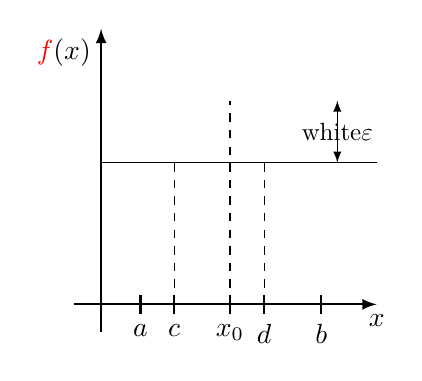
\begin{tikzpicture}

\tikzset{>=latex} % for LaTeX arrow head

  \def\tick#1#2{\draw[thick] (#1)++(#2:0.12) --++ (#2-180:0.24)}
 \def\N{100} % number of samples

  \def\xmax{3.5}
  \def\ymax{3.5}
  \def\xeps{3}
  \def\yeps{1.8}
  \coordinate (O) at (0,0);
  \coordinate (C) at (0.927575,0);
  \coordinate (A) at (0.5,0);
  \coordinate (B) at (2.796001,0);
  \coordinate (D) at (2.0700,0);
  \coordinate (X0) at (1.63694,0);
  \def\yMAX{2.587020}

  % AXIS
  \draw[->,thick]
    (-0.1*\ymax,0) -- (\xmax,0) node[below] {$x$};
    \draw[->,thick] (0,-0.1*\ymax) -- (0,\ymax) node[below left] {$\textcolor{red}{f}(x)$};
  
  % PLOT
  % \draw[xline,red,samples=\N,smooth,variable=\x,domain=-0.1:0.94*\xmax,thick]   plot(\x,{3/(1+(0.36*\x*\x-1)^2) -\x/4});
    
  \draw[dashed,thin] (X0) --++ (0,\yMAX);
  \draw[dashed,thin] (C) --++ (0,\yeps);
  \draw[dashed,thin] (D) --++ (0,\yeps);
  
  % \draw[thin] (0,\yMAX) -- (\xmax,\yMAX) node[left] at (0,\yMAX) {$M$};
  \draw[thin] (0,\yeps) -- (\xmax,\yeps);
  
  \draw[<->] (\xeps,\yeps) -- (\xeps,\yMAX)
    node[midway,scale=0.9] {\contour{white}{$\varepsilon$}};
    
  \tick{X0}{90} node[below] {$x_0$};
  \tick{A}{90} node[below] {$a$};
  \tick{B}{90} node[below] {$b$};
  \tick{C}{90} node[below] {$c$};
  \tick{D}{90} node[below] {$d$};
  
\end{tikzpicture}

    \caption{Illustration à finir}
\end{figure}
% \end{comment}

\subsection{Limite $p \to 0$}

\begin{theo}
Soit $f \in \mathscr{C}([0,1],\R^*)$. Alors,
\[
\lim_{p\to0} \norm{f}_{L^p} = \exp\left\{\int_0^1 \ln\module{f(x)} \d x\right\}.
\]
\end{theo}

%---------------

\begin{exercice}%
Soit $f \in \mathscr{C}([0,1],\R^\ast)$. On suppose que $f$ est à valeurs positives et on pose $I(y) = \int_0^1 f(x)^y \d x$.
\begin{questions}
\item Soit $g$ une fonction définie sur un voisinage de $0$ à valeurs dans $\R_+^\ast$, dérivable en $0$, vérifiant $g(0) = 1$. Déterminer $\lim\limits_{y\to0} g(y)^{1/y}$.

\item Montrer que $I$ est une fonction dérivable sur $\R_+$.

\item En déduire que
\[
\lim_{y\to0} \left(\int_0^1 f(x)^y \d x\right)^{1/y} = \exp\left\{\int_0^1 \ln(f(x)) \d x\right\}.
\]
\end{questions}
\end{exercice}

\begin{solution}
\begin{reponses}
\item Comme $g$ est dérivable, d'après le théorème de Taylor-Young, $g(y) = 1 + y g'(0) + o(y)$. Ainsi,
\begin{align*}
g(y)^{1/y} &= \exp\left\{\frac{1}{y} \ln(g(0) + y g'(0) + o(y))\right\}
= \exp\left\{g'(0) + o(1)\right\}
\to \e^{g'(0)}.
\end{align*}

\item En posant $F: (x, y) \mapsto f(x)^y$, alors
\[
\abs{\frac{\partial F}{\partial y}(x, y)} = \abs{\ln(f(x)) f(x)^y}.
\]

La fonction $\ln \circ f$ est continue sur le segment $[0, 1]$ donc elle est bornée par une constante $M$. Ainsi,
\begin{align*}
\module{F(x, y)} &\leq \e^{a M},\\
\module{\frac{\partial F}{\partial y}(x, y)} &\leq M \cdot \e^{a M}.
\end{align*}

D'après le théorème de dérivation sous le signe intégral, la fonction $I$ est dérivable sur $[0, 1[$ et
\begin{align*}
I'(y) &= \int_0^1 \ln(f(x)) f(x)^y \d x \\
I'(0) &= \int_0^1 \ln(f(x)) \d x
\end{align*}

\item Finalement,
\[
\lim_{y\to0} \left(\int_0^1 f(x)^y \d x\right)^{1/y} = \exp\left\{\int_0^1 \ln(f(x)) \d x\right\}.
\]
\end{reponses}
\end{solution}

\url{https://math.stackexchange.com/questions/2351581/convergence-question-about-lp-norm-when-p-tends-to-zero}


%-----------
\subsection{Cas $p \geq 1$}

Lorsque l'exposant $p$ satisfait $0 < p < 1$, on constate que l'inégalité triangulaire ne peut pas être satisfaite par $\norm{\cdot}_{L^p}$, ce qui justifie, pour bénéficier d’une structure naturelle d’espace vectoriel, de se restreindre à supposer $1 < p < +\infty$.

\begin{theo}[Inégalité de \textsc{Minkowski}]
Soit $p \geq 1$. Si $f$ et $g$ sont deux fonctions appartenant à $L^p(I)$, alors
\[
\norm{f + g}_{L^p} \leq \norm{f}_{L^p} + \norm{g}_{L^p}.
\]
Ainsi, $L^p(I)$ est un espace vectoriel et $\norm{\cdot}_{L^p}$ est une norme.
\end{theo}

\begin{remarque}
Les cas $p = 1$ et $p = +\infty$ sont aisément vérifiables. On se limite par la suite au cas $1 < p < +\infty$.
\end{remarque}

Cette inégalité repose sur le théorème suivant :
\begin{theo}[Inégalité de \textsc{Hölder}]
Soient $1 < p,\, q < +\infty$, $q$ tels que $\frac{1}{p} + \frac{1}{q} = 1$ et $f,\, g$ deux fonctions à valeurs strictement positives. Si $f$ appartient à $L^p(I)$ et $g \in L^q(I)$, alors $f g$ appartient à $L^1(I)$ et
\[
\int_I f g \leq \norm{f}_{L^p} \norm{g}_{L^q}.
\]
\end{theo}

\begin{remarque}
Lorsque $p = 2$, alors $q = 2$ et on retrouve l'inégalité de Cauchy-Schwarz.
\end{remarque}

\begin{exercice}
Les cas où $\norm{f}_{L^p} = 0$ ou $\norm{g}_{L^q} = 0$ sont triviaux. On se limite donc au cas où ces quantités sont non nulles et on pose
\[
F = \frac{f}{\norm{f}_{L^p}}
\text{ et }
G = \frac{g}{\norm{g}_{L^q}}.
\]
Soit $x \in I$.
\begin{questions}
\item Montrer qu'il existe deux réels $s$ et $t$ tels que $F(x) = \e^{t/p}$ et $G(x) = \e^{s/q}$.

\item Montrer que $\e^{\frac{s}{p} + \frac{t}{q}} \leq \frac{1}{p} \e^s + \frac{1}{q} \e^t$.

\item En déduire l'inégalité de Hölder.
\end{questions}
\end{exercice}

\begin{solution}
\begin{reponses}
\item Pour tout $x$ réel, $F(x)$ et $G(x)$ sont deux réels strictement positifs, on pose $t = p \ln(F(x))$ et $s = q \ln(G(x))$.

\item Rappelons que $\frac{1}{p} + \frac{1}{q} = 1$. Pour tous $s$ et $t$ réels, comme la fonction exponentielle est convexe, d'après l'inégalité de Jensen,
\[
\e^{\frac{s}{p} + \frac{t}{q}} \leq \frac{1}{p} \e^s + \frac{1}{q} \e^t.
\]

\item Alors,
\begin{align*}
F(x) G(x) &\leq \frac{1}{p} F(x)^p + \frac{1}{q} G(x)^q
\end{align*}
Comme $F^p$ et $G^q$ sont intégrables, alors $F G$ est intégrable et
\[
\int_I F G \leq \frac{1}{p} + \frac{1}{q} = 1.
\]
La linéarité de l'intégrale permet alors de conclure.
\end{reponses}
\end{solution}

\begin{exercice}
Soit $f$ et $g$ deux fonctions de classe $L^p$ sur $I$.
\begin{questions}
\item Montrer que $\module{f + g}^p \leq 2^p \module{f}^p + 2^p \module{g}^p$.

\item En déduire que $(f + g) \in L^p(I)$.

\item En décomposant $(f + g)^p = f (f + g)^{p-1} + g (f + g)^{p-1}$, en déduire l'inégalité de Minkowski.
\end{questions}
\end{exercice}

\begin{solution}
\begin{reponses}
\item Pour tout $x \in I$,
\begin{itemize}
\item soit $\module{f(x)} \leq \module{g(x)}$ et $\module{f(x) + g(x)}^p \leq 2^p \module{g(x)}^p$,
\item soit $\module{g(x)} \leq \module{f(x)}$ et $\module{f(x) + g(x)}^p \leq 2^p \module{f(x)}^p$.
\end{itemize}
Ainsi, dans tous les cas,
\[
\module{f + g}^p \leq 2^p \module{f}^p + 2^p \module{g}^p.
\]

\item D'après la question précédente et le théorème de comparaison des intégrales, $f + g \in L^p(I)$.

\item En utilisant la décomposition proposée, on remarque que
\begin{align*}
\left(\module{f + g}^{p-1}\right)^q
&= \module{f + g}^{q(p-1)}
= \module{f + g}^p.
\end{align*}
Ainsi, $\module{f + g}^{p-1} \in L^q(I)$.

En appliquant deux fois l'inégalité de Hölder,
\begin{align*}
\norme{f + g}_{L^p}^p
&= \norme{|f| \cdot |f + g|^{p-1}}_{L^1}
+ \norme{|g| \cdot |f + g|^{p-1}}_{L^1}\\
&\leq \norm{f}_{L^p}^p \norm{f + g}_{L^p}^{p/q}
+ \norm{g}_{L^p}^p \norm{f + g}_{L^p}^{p/q}\\
&\leq \norm{f + g}_{L^p}^{p/q} \left(\norm{f}_{L^p} + \norm{f}_{L^q}\right).
\end{align*}

On conclut en simplifiant par $\norm{f + g}_{L^p}^{p/q}$.
\end{reponses}
\end{solution}

\todoinline{Pointer vers
Exercice 2 de \url{https://www.imo.universite-paris-saclay.fr/~joel.merker/Enseignement/Integration/l-p-espaces.pdf}}
% \begin{exercice}
    % On considère les espaces $L^p(\R^d)$ pour  $0 < p < +\infty$. Montrer que si l'on a 
    % \[
    % \norm{f + g}_{L^p} \leqslant  \norm{f}_{L^p} + \norm{g}_{L^p}
    % \]
    % pour toutes fonctions $f, g \in L^p(\R^d )$, alors nécessairement $p \geqslant 1$.
% \end{exercice}

%-----------
\subsection{Inclusions entre les $L^p$}

\begin{theo}
Si $I$ est un intervalle borné, on note $|I|$ sa longueur. Pour tout $p < q$, $L^q(I) \subset L^p(I)$ et $\|f\|_p \leq \module{I}^{\frac{1}{p} - \frac{1}{q}} \norm{f}_{L^q}$.
    % Si $\Omega$ est de mesure $\module{\Omega}$ finie, alors pour $p<q$, $L^q(\Omega) \subset L^p(\Omega)$ et pour tout $f \in L^q(\Omega)$, $\norm{f}_{L^p} \leqslant \module{\Omega}^{\frac{1}{p} - \frac{1}{q}} \norm{f}_{L^q}$.
\end{theo}

\begin{demo}
Comme $I$ est borné, alors la fonction constante égale à $1$ appartient à tous les espaces $L^q$. Ainsi, d'après l'inégalité de Hölder,
\begin{align*}
\norm{f}_{L^p}^p
&\leq \left(\int_I \module{f}^q\right)^{p/q} \left(\int_I 1\right)^{1-p/q}
\leq \norm{f}_{L^q}^p \cdot \module{I}^{1-p/q}.
\end{align*}
\end{demo}

\begin{remarque}
En utilisant des intégrales de Riemann, on montre que ces inclusions sont fausses dès que $I$ n'est pas borné. \\
En effet, choisissons $p$ et $q$ tels que $p > q$ et considérons $\alpha > 0$ avec la fonction $f(x) = \frac{1}{1+\module{x}^\alpha}$ pour $x \in \R$. Si on choisit $1/p < \alpha < 1/q$, alors $f \in L^p(\R)$ mais $f \not\in L^q(\R)$, donc $L^p(\R) \not\subset L^q(\R)$. \\
Considérons maintenant la fonction $g(x) = \frac{1}{\module{x}^\alpha (1+x^2)}$ pour $x \in \R$. Si on choisit encore $\alpha$ tel que $1/p <  \alpha < 1/q$, alors $g \in L^q(\R)$ mais $g \not\in L^p(\R)$, donc $L^q(\R) \not\subset L^p(\R)$.
\end{remarque}

\todoinline{Pointer vers Rudin pour une caractérisation des inclusions}